% ------------------------------------------------------------------------------
% 5.4. DETALLE DE CASOS DE USO
% Cada CU: (1) diagrama de contexto [pendiente de insertar] y (2) tabla de detalle.
% ------------------------------------------------------------------------------
% Listas compactas para las celdas de las tablas de detalle.
\newenvironment{cupasos}{\begin{enumerate}\setlength{\itemsep}{1pt}\setlength{\topsep}{2pt}\setlength{\parsep}{0pt}\setlength{\parskip}{0pt}\setlength{\leftmargin}{1.5em}}{\end{enumerate}}
\newenvironment{cuvin}{\begin{itemize}\setlength{\itemsep}{1pt}\setlength{\topsep}{2pt}\setlength{\parsep}{0pt}\setlength{\parskip}{0pt}\setlength{\leftmargin}{1.2em}}{\end{itemize}}

\subsection{5.4. Detalle de Casos de Uso}\label{sec:cap5_detalle_cu}

\subsubsection{5.4.1. CU-01 Registrarse y autenticarse}\label{sec:cap5_cu01}

\begin{figure}[H]
\caption{Diagrama de contexto del CU-01}
\label{fig:ctx_cu01}
\centering
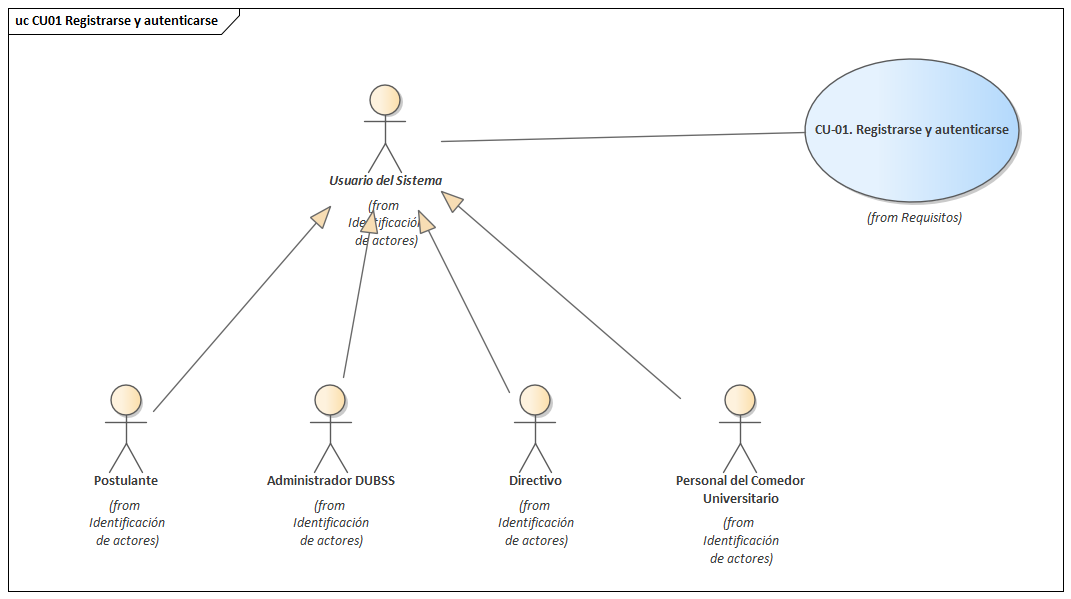
\includegraphics[width=0.8\textwidth,height=0.4\textheight,keepaspectratio]{images/038_CU01_Registrarse_Autenticarse.png}

\smallskip
\noindent\raggedright\textit{Nota.} Elaboración propia.
\end{figure}

\refstepcounter{table}\label{tab:detalle_cu01}
\addcontentsline{lot}{table}{\protect\numberline{\thetable}Detalle del CU-01: Registrarse y autenticarse}
\noindent\textbf{Tabla~\thetable}\par\nopagebreak
\noindent\textit{Detalle del CU-01: Registrarse y autenticarse}\par\nopagebreak
\begingroup\small\linespread{1}\selectfont
\begin{longtable}{>{\raggedright\arraybackslash}p{2.9cm} >{\raggedright\arraybackslash}p{12.6cm}}
\toprule
\textbf{Caso de Uso} & \textbf{CU-01. Registrarse y autenticarse} \\
\midrule
\endfirsthead
\toprule
\textbf{Caso de Uso} & \textbf{CU-01. Registrarse y autenticarse} \\
\midrule
\endhead
\endfoot
\bottomrule
\multicolumn{2}{l}{\textit{Nota.} Elaboración propia.} \\
\endlastfoot
\textbf{Propósito} & Permitir que los usuarios del sistema se registren (en el caso del Postulante) y se autentiquen para acceder, de forma segura, a las funcionalidades correspondientes a su rol, desde el portal web o la aplicación móvil. \\
\midrule
\textbf{Descripción} & Este caso de uso describe cómo un Postulante crea su cuenta y cómo cualquier usuario del sistema (Postulante, Administrador DUBSS, Directivo o Personal del Comedor Universitario) inicia sesión con su correo electrónico y contraseña mediante autenticación basada en JWT (JSON Web Token) gestionada por el backend. Una vez autenticado, el sistema identifica el rol del usuario y lo redirige al módulo que le corresponde. Las cuentas del personal (Administrador, Directivo y Personal del Comedor) no se autorregistran: son creadas por el Administrador DUBSS en el CU-14. El CU-15 extiende este caso de uso para la recuperación de contraseña. Respalda el RF-01. \\
\midrule
\textbf{Actores} & Usuario del Sistema (Postulante, Administrador DUBSS, Directivo, Personal del Comedor Universitario). \\
\midrule
\textbf{Actor Iniciador} & Usuario del Sistema. \\
\midrule
\textbf{Precondición} & \vspace{-\baselineskip}\begin{cuvin}
    \item El usuario dispone de acceso al portal web o a la aplicación móvil y de conexión a Internet.
    \item Para el registro: el postulante no cuenta con una cuenta asociada a su CI ni a su correo electrónico.
    \item Para la autenticación: el usuario cuenta con una cuenta registrada y activa en el sistema.
\end{cuvin} \\
\midrule
\textbf{Proceso} & \textbf{Flujo principal A: registro de un Postulante.}
\begin{cupasos}
    \item El usuario selecciona la opción «Crear cuenta» en la pantalla de acceso.
    \item El sistema muestra el formulario de registro (nombres, apellidos, CI, carrera, correo electrónico, contraseña y confirmación de contraseña).
    \item El usuario completa los datos y confirma el registro.
    \item El sistema valida que los campos obligatorios estén completos, que su formato sea correcto, que la contraseña cumpla la política de seguridad (por definir con la DUBSS) y que el CI y el correo electrónico no existan en el sistema.
    \item El sistema registra al usuario con el rol Postulante en la base de datos, almacenando la contraseña de forma cifrada (hash).
    \item El sistema informa que el registro fue exitoso, inicia la sesión del usuario y lo redirige al módulo del Postulante.
\end{cupasos} \\
 & \textbf{Flujo principal B: inicio de sesión.}
\begin{cupasos}
    \item El usuario accede a la pantalla de inicio de sesión del portal web o de la aplicación móvil.
    \item El usuario ingresa su correo electrónico y su contraseña.
    \item El sistema envía las credenciales al backend, que las valida comparando la contraseña ingresada con el hash almacenado.
    \item El sistema verifica que la cuenta esté activa y obtiene el rol del usuario.
    \item El sistema genera un token JWT firmado, con el identificador y el rol del usuario y una fecha de expiración, lo entrega al cliente para autenticar las siguientes peticiones y redirige al usuario según su rol: el Postulante a su módulo de postulación, el Administrador DUBSS al panel de gestión, el Directivo al dashboard de indicadores y el Personal del Comedor al registro de asistencia.
\end{cupasos} \\
 & \textbf{Flujos alternativos.}
\begin{cuvin}
    \item A1 (flujo A, paso 4): si el CI o el correo electrónico ya están registrados, el sistema rechaza el registro e indica el campo en conflicto, sin crear la cuenta.
    \item A2 (flujo A, paso 4): si faltan campos obligatorios, el formato es inválido o la contraseña no cumple la política, el sistema marca los campos con error y permite corregirlos.
    \item A3 (flujo B, paso 3): si las credenciales son incorrectas, el sistema muestra un mensaje de error genérico (sin revelar cuál dato falló) y permite reintentar.
    \item A4 (flujo B, paso 4): si la cuenta está desactivada, el sistema niega el acceso e indica que debe comunicarse con la DUBSS.
    \item A5 (flujo B, paso 2): si el usuario selecciona «¿Olvidó su contraseña?», se ejecuta el CU-15.
    \item A6 (flujo B, paso 3): tras un número de intentos fallidos consecutivos (límite por definir con la DUBSS), el sistema bloquea temporalmente el acceso de esa cuenta.
\end{cuvin} \\
\midrule
\textbf{Postcondición} & \vspace{-\baselineskip}\begin{cuvin}
    \item Registro: la cuenta del Postulante queda creada en la base de datos con el rol Postulante.
    \item Autenticación: el usuario tiene una sesión activa con los permisos de su rol y el acceso queda registrado en el log del sistema.
\end{cuvin} \\
\midrule
\textbf{Excepciones} & \vspace{-\baselineskip}\begin{cuvin}
    \item Credenciales inválidas o cuenta inexistente.
    \item Cuenta desactivada o bloqueada temporalmente.
    \item Token de sesión inválido o sesión expirada.
    \item Error de conexión con el servidor o la base de datos.
    \item Petición de registro duplicada (se procesa de forma idempotente, sin crear dos cuentas).
\end{cuvin} \\
\end{longtable}
\endgroup
\addtocounter{table}{-1}

\subsubsection{5.4.2. CU-02 Enviar postulación a Beca Comedor}\label{sec:cap5_cu02}

\begin{figure}[H]
\caption{Diagrama de contexto del CU-02}
\label{fig:ctx_cu02}
\centering
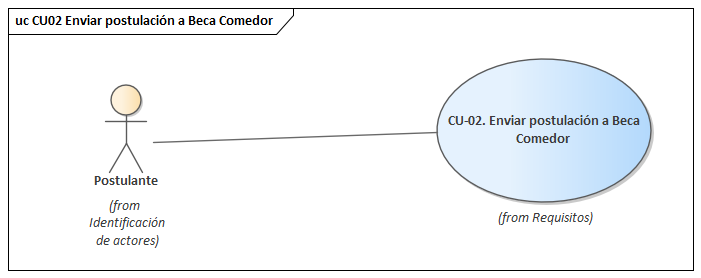
\includegraphics[width=0.8\textwidth,height=0.4\textheight,keepaspectratio]{images/039_CU02_Enviar_Postulacion_Beca_Comedor.png}

\smallskip
\noindent\raggedright\textit{Nota.} Elaboración propia.
\end{figure}

\refstepcounter{table}\label{tab:detalle_cu02}
\addcontentsline{lot}{table}{\protect\numberline{\thetable}Detalle del CU-02: Enviar postulación a Beca Comedor}
\noindent\textbf{Tabla~\thetable}\par\nopagebreak
\noindent\textit{Detalle del CU-02: Enviar postulación a Beca Comedor}\par\nopagebreak
\begingroup\small\linespread{1}\selectfont
\begin{longtable}{>{\raggedright\arraybackslash}p{2.9cm} >{\raggedright\arraybackslash}p{12.6cm}}
\toprule
\textbf{Caso de Uso} & \textbf{CU-02. Enviar postulación a Beca Comedor} \\
\midrule
\endfirsthead
\toprule
\textbf{Caso de Uso} & \textbf{CU-02. Enviar postulación a Beca Comedor} \\
\midrule
\endhead
\endfoot
\bottomrule
\multicolumn{2}{l}{\textit{Nota.} Elaboración propia.} \\
\endlastfoot
\textbf{Propósito} & Permitir al Postulante completar el formulario socioeconómico, adjuntar su documentación digitalizada y enviar formalmente su postulación a la Beca Comedor de la convocatoria vigente. \\
\midrule
\textbf{Descripción} & Este caso de uso describe cómo el Postulante registra su postulación desde el portal web o la aplicación móvil. Incluye la digitalización y carga de documentos (CU-16), la validación de elegibilidad y duplicados (CU-18) y la precalificación automática con Inteligencia Artificial (CU-03). El CU-17 lo extiende para guardar la postulación como borrador. Respalda el RF-02. \\
\midrule
\textbf{Actores} & Postulante. \\
\midrule
\textbf{Actor Iniciador} & Postulante. \\
\midrule
\textbf{Precondición} & \vspace{-\baselineskip}\begin{cuvin}
    \item El Postulante está autenticado en el sistema (CU-01).
    \item Existe una convocatoria abierta (CU-13) para la gestión académica vigente.
    \item El Postulante no tiene otra postulación vigente en la misma gestión, salvo que la suya haya sido devuelta para corrección (CU-19).
    \item El Postulante dispone de los documentos obligatorios definidos en la convocatoria.
\end{cuvin} \\
\midrule
\textbf{Proceso} & \textbf{Flujo principal.}
\begin{cupasos}
    \item El Postulante selecciona la opción «Nueva postulación».
    \item El sistema verifica que exista una convocatoria abierta y muestra el formulario socioeconómico con los datos del perfil precargados (nombre, CI y carrera).
    \item El Postulante completa las variables socioeconómicas: ingresos familiares, número de dependientes, procedencia, patrimonio, estado de vulnerabilidad y promedio académico.
    \item El Postulante digitaliza o adjunta los documentos de respaldo requeridos (se incluye el CU-16).
    \item El Postulante selecciona «Enviar postulación».
    \item El sistema verifica que no falte ningún campo ni documento obligatorio y que los datos tengan un formato válido.
    \item El sistema valida la elegibilidad del Postulante y la inexistencia de duplicados (se incluye el CU-18).
    \item El sistema registra la postulación con estado «pendiente», asociándola a la convocatoria y gestión académica vigentes, con su fecha y hora de envío.
    \item El sistema solicita la precalificación de la postulación (se incluye el CU-03).
    \item El sistema confirma la recepción de la postulación y muestra al Postulante un comprobante con su código de postulación.
\end{cupasos} \\
 & \textbf{Flujos alternativos.}
\begin{cuvin}
    \item A1 (paso 1): si no existe una convocatoria abierta, el sistema impide iniciar la postulación e informa las fechas de la próxima convocatoria, si están definidas.
    \item A2 (pasos 3 y 4): si el Postulante desea continuar más tarde, puede guardar su avance como borrador (CU-17).
    \item A3 (paso 6): si faltan campos o documentos obligatorios, el sistema resalta lo faltante y no permite enviar la postulación.
    \item A4 (paso 7): si el Postulante no es elegible o ya tiene una postulación vigente en la gestión, el sistema rechaza el envío e informa el motivo.
    \item A5 (paso 1): si el Postulante tiene una postulación en estado «devuelta», el sistema le permite abrirla, corregirla y reenviarla; esta no se considera duplicada y se conserva el historial de devoluciones y reenvíos.
    \item A6 (paso 5): si el Postulante presiona repetidamente el botón de envío o la petición llega duplicada, el sistema la procesa una sola vez (idempotencia).
    \item A7 (paso 9): si el módulo de IA no responde, la postulación queda registrada con estado «pendiente» y la precalificación se reintenta automáticamente; el Postulante no pierde su envío.
    \item A8 (pasos 2 a 5): si la convocatoria se cierra mientras el Postulante completa el formulario, el sistema no acepta el envío e informa que el plazo finalizó.
\end{cuvin} \\
\midrule
\textbf{Postcondición} & \vspace{-\baselineskip}\begin{cuvin}
    \item La postulación queda almacenada con estado «pendiente» (o «calificada» una vez ejecutado el CU-03), asociada al Postulante, a la convocatoria y a la gestión académica.
    \item Los documentos adjuntos quedan almacenados en Firebase Storage y vinculados a la postulación.
    \item El Postulante puede consultar el estado de su postulación (CU-04).
\end{cuvin} \\
\midrule
\textbf{Excepciones} & \vspace{-\baselineskip}\begin{cuvin}
    \item Autenticación inválida o sesión expirada.
    \item Falta de permisos suficientes (el usuario no tiene el rol Postulante).
    \item Datos ingresados no válidos o campos obligatorios incompletos.
    \item Convocatoria cerrada o inexistente.
    \item Postulación duplicada o Postulante no elegible.
    \item Error al almacenar los archivos en Firebase Storage.
    \item Error de conexión con el servidor o la base de datos durante el envío.
\end{cuvin} \\
\end{longtable}
\endgroup
\addtocounter{table}{-1}

\subsubsection{5.4.3. CU-03 Precalificar postulación con Inteligencia Artificial}\label{sec:cap5_cu03}

\begin{figure}[H]
\caption{Diagrama de contexto del CU-03}
\label{fig:ctx_cu03}
\centering
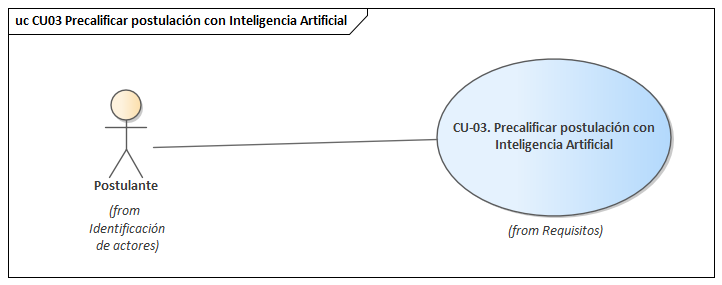
\includegraphics[width=0.8\textwidth,height=0.4\textheight,keepaspectratio]{images/040_CU03_Precalificar_Postulacion_IA.png}

\smallskip
\noindent\raggedright\textit{Nota.} Elaboración propia.
\end{figure}

\refstepcounter{table}\label{tab:detalle_cu03}
\addcontentsline{lot}{table}{\protect\numberline{\thetable}Detalle del CU-03: Precalificar postulación con Inteligencia Artificial}
\noindent\textbf{Tabla~\thetable}\par\nopagebreak
\noindent\textit{Detalle del CU-03: Precalificar postulación con Inteligencia Artificial}\par\nopagebreak
\begingroup\small\linespread{1}\selectfont
\begin{longtable}{>{\raggedright\arraybackslash}p{2.9cm} >{\raggedright\arraybackslash}p{12.6cm}}
\toprule
\textbf{Caso de Uso} & \textbf{CU-03. Precalificar postulación con Inteligencia Artificial} \\
\midrule
\endfirsthead
\toprule
\textbf{Caso de Uso} & \textbf{CU-03. Precalificar postulación con Inteligencia Artificial} \\
\midrule
\endhead
\endfoot
\bottomrule
\multicolumn{2}{l}{\textit{Nota.} Elaboración propia.} \\
\endlastfoot
\textbf{Propósito} & Calcular automáticamente, mediante un modelo de Inteligencia Artificial, el puntaje de vulnerabilidad de cada postulación recibida, para ordenar objetivamente a los postulantes según su nivel de necesidad. \\
\midrule
\textbf{Descripción} & Este caso de uso describe cómo el sistema precalifica cada postulación enviada, enviando sus variables socioeconómicas y académicas al módulo de IA (desarrollado en Python y consumido mediante API) y registrando el puntaje obtenido junto con su fecha de cálculo. El puntaje permite construir la lista priorizada que usa el Administrador DUBSS para auditar únicamente a los finalistas (CU-06). Es incluido por el CU-02 y extendido por el CU-26, que permite reprocesar los puntajes. Respalda el RF-03. \\
\midrule
\textbf{Actores} & Postulante. \\
\midrule
\textbf{Actor Iniciador} & Postulante (a través del CU-02, al enviar su postulación; el sistema ejecuta la precalificación mediante el módulo de IA). \\
\midrule
\textbf{Precondición} & \vspace{-\baselineskip}\begin{cuvin}
    \item La postulación fue enviada, superó la validación de elegibilidad y duplicados (CU-18) y se encuentra en estado «pendiente».
    \item El módulo de IA está disponible y tiene cargados los parámetros vigentes del modelo (criterios y ponderaciones por definir con la DUBSS).
    \item La postulación contiene las variables requeridas por el modelo: ingresos familiares, dependientes, procedencia, carrera, patrimonio, estado de vulnerabilidad y promedio académico.
\end{cuvin} \\
\midrule
\textbf{Proceso} & \textbf{Flujo principal.}
\begin{cupasos}
    \item El sistema (backend) detecta una postulación pendiente de precalificar y prepara el conjunto de variables socioeconómicas y académicas declaradas.
    \item El sistema envía la solicitud de cálculo al módulo de IA mediante la API.
    \item El módulo de IA valida que los datos recibidos estén completos y sean consistentes.
    \item El módulo de IA aplica el modelo con los parámetros vigentes y calcula el puntaje de vulnerabilidad.
    \item El módulo de IA devuelve el puntaje al sistema.
    \item El sistema registra el puntaje junto con la fecha y hora de cálculo y la versión de los parámetros utilizados, conservando los puntajes anteriores si existieran.
    \item El sistema actualiza el estado de la postulación a «calificada» e incorpora la postulación a la lista priorizada.
\end{cupasos} \\
 & \textbf{Flujos alternativos.}
\begin{cuvin}
    \item A1 (paso 3): si los datos están incompletos o son inconsistentes, el módulo de IA no calcula el puntaje; el sistema registra el error y deja la postulación marcada para revisión.
    \item A2 (paso 2): si el módulo de IA no está disponible o excede el tiempo de espera, el sistema registra el fallo, mantiene la postulación en estado «pendiente» y reintenta el cálculo automáticamente.
    \item A3 (paso 1): si la solicitud proviene del reprocesamiento (CU-26), el sistema calcula un nuevo puntaje con los parámetros actualizados y conserva el puntaje anterior para trazabilidad.
    \item A4 (paso 1): si se recibe una solicitud duplicada para la misma postulación y la misma versión de parámetros, el sistema no genera un segundo puntaje (idempotencia).
    \item A5 (paso 1): ante picos de envíos (por ejemplo, al cierre de la convocatoria), el sistema encola las solicitudes y las procesa en orden, de modo que la totalidad de las postulaciones (hasta 20,000 por gestión) sea procesada sin intervención manual.
\end{cuvin} \\
\midrule
\textbf{Postcondición} & \vspace{-\baselineskip}\begin{cuvin}
    \item Cada postulación procesada tiene un puntaje de vulnerabilidad registrado con su fecha de cálculo, lo que permite su trazabilidad.
    \item La postulación queda en estado «calificada» y disponible en la lista priorizada (CU-06).
\end{cuvin} \\
\midrule
\textbf{Excepciones} & \vspace{-\baselineskip}\begin{cuvin}
    \item Módulo de IA no disponible o tiempo de espera agotado (el cálculo individual debe completarse en un máximo de 5 segundos en condiciones normales).
    \item Datos de la postulación incompletos o inconsistentes.
    \item Error en la comunicación entre el backend y el módulo de IA.
    \item Error de conexión con la base de datos al registrar el puntaje.
\end{cuvin} \\
\end{longtable}
\endgroup
\addtocounter{table}{-1}

\subsubsection{5.4.4. CU-04 Consultar estado de postulación}\label{sec:cap5_cu04}

\begin{figure}[H]
\caption{Diagrama de contexto del CU-04}
\label{fig:ctx_cu04}
\centering
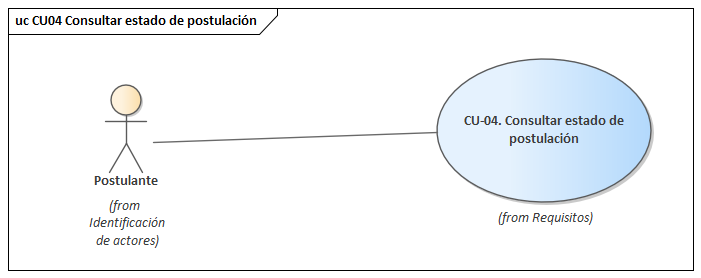
\includegraphics[width=0.8\textwidth,height=0.4\textheight,keepaspectratio]{images/041_CU04_Consultar_Estado_Postulacion.png}

\smallskip
\noindent\raggedright\textit{Nota.} Elaboración propia.
\end{figure}

\refstepcounter{table}\label{tab:detalle_cu04}
\addcontentsline{lot}{table}{\protect\numberline{\thetable}Detalle del CU-04: Consultar estado de postulación}
\noindent\textbf{Tabla~\thetable}\par\nopagebreak
\noindent\textit{Detalle del CU-04: Consultar estado de postulación}\par\nopagebreak
\begingroup\small\linespread{1}\selectfont
\begin{longtable}{>{\raggedright\arraybackslash}p{2.9cm} >{\raggedright\arraybackslash}p{12.6cm}}
\toprule
\textbf{Caso de Uso} & \textbf{CU-04. Consultar estado de postulación} \\
\midrule
\endfirsthead
\toprule
\textbf{Caso de Uso} & \textbf{CU-04. Consultar estado de postulación} \\
\midrule
\endhead
\endfoot
\bottomrule
\multicolumn{2}{l}{\textit{Nota.} Elaboración propia.} \\
\endlastfoot
\textbf{Propósito} & Permitir al Postulante realizar el seguimiento del estado de su postulación sin necesidad de acudir presencialmente a la DUBSS. \\
\midrule
\textbf{Descripción} & Este caso de uso describe cómo el Postulante consulta, desde el portal web o la aplicación móvil, el estado actual de sus postulaciones, el historial de cambios y, según corresponda, las observaciones de devolución, el motivo de archivo o rechazo y el resultado de la adjudicación. Cuando el estado cambia, el sistema notifica al Postulante mediante notificación push y la notificación lo dirige a esta consulta. Es una consulta de solo lectura. Respalda el RF-06. \\
\midrule
\textbf{Actores} & Postulante. \\
\midrule
\textbf{Actor Iniciador} & Postulante. \\
\midrule
\textbf{Precondición} & \vspace{-\baselineskip}\begin{cuvin}
    \item El Postulante está autenticado en el sistema (CU-01).
    \item El Postulante ha enviado al menos una postulación.
\end{cuvin} \\
\midrule
\textbf{Proceso} & \textbf{Flujo principal.}
\begin{cupasos}
    \item El Postulante accede a la opción «Mis postulaciones».
    \item El sistema muestra la lista de sus postulaciones con la gestión académica, la fecha de envío y el estado actual.
    \item El Postulante selecciona una postulación.
    \item El sistema muestra el detalle: estado actual (pendiente, devuelta, archivada, calificada, adjudicada o no adjudicada), historial de cambios de estado con fecha y hora, y la información asociada al estado.
    \item El Postulante revisa la información y, si lo desea, regresa a la lista.
\end{cupasos} \\
 & \textbf{Flujos alternativos.}
\begin{cuvin}
    \item A1 (paso 2): si el Postulante no tiene postulaciones, el sistema muestra un mensaje informativo e invita a postular si existe una convocatoria abierta.
    \item A2 (paso 2): si el Postulante tiene postulaciones de varias gestiones, el sistema permite filtrarlas por gestión académica.
    \item A3 (paso 4): si la postulación está «devuelta», el sistema muestra las observaciones registradas por el Administrador (CU-19) y ofrece la opción de corregir y reenviar (CU-02).
    \item A4 (paso 4): si la postulación está «archivada» o «no adjudicada», el sistema muestra el motivo registrado (CU-20).
    \item A5 (paso 4): si el Postulante fue seleccionado como finalista, el sistema muestra la notificación con el plazo y los documentos físicos que debe presentar (CU-21); si los resultados fueron publicados, muestra su resultado (CU-22).
    \item A6 (paso 1): si el Postulante accede desde una notificación push, el sistema abre directamente el detalle de la postulación afectada.
\end{cuvin} \\
\midrule
\textbf{Postcondición} & \vspace{-\baselineskip}\begin{cuvin}
    \item El Postulante visualiza el estado actualizado de su postulación; la consulta no modifica ningún dato del sistema.
\end{cuvin} \\
\midrule
\textbf{Excepciones} & \vspace{-\baselineskip}\begin{cuvin}
    \item Autenticación inválida o sesión expirada.
    \item Falta de permisos suficientes (el Postulante solo puede consultar sus propias postulaciones).
    \item Error de conexión con el servidor o la base de datos.
\end{cuvin} \\
\end{longtable}
\endgroup
\addtocounter{table}{-1}

\subsubsection{5.4.5. CU-05 Auditar y adjudicar becas}\label{sec:cap5_cu05}

\begin{figure}[H]
\caption{Diagrama de contexto del CU-05}
\label{fig:ctx_cu05}
\centering
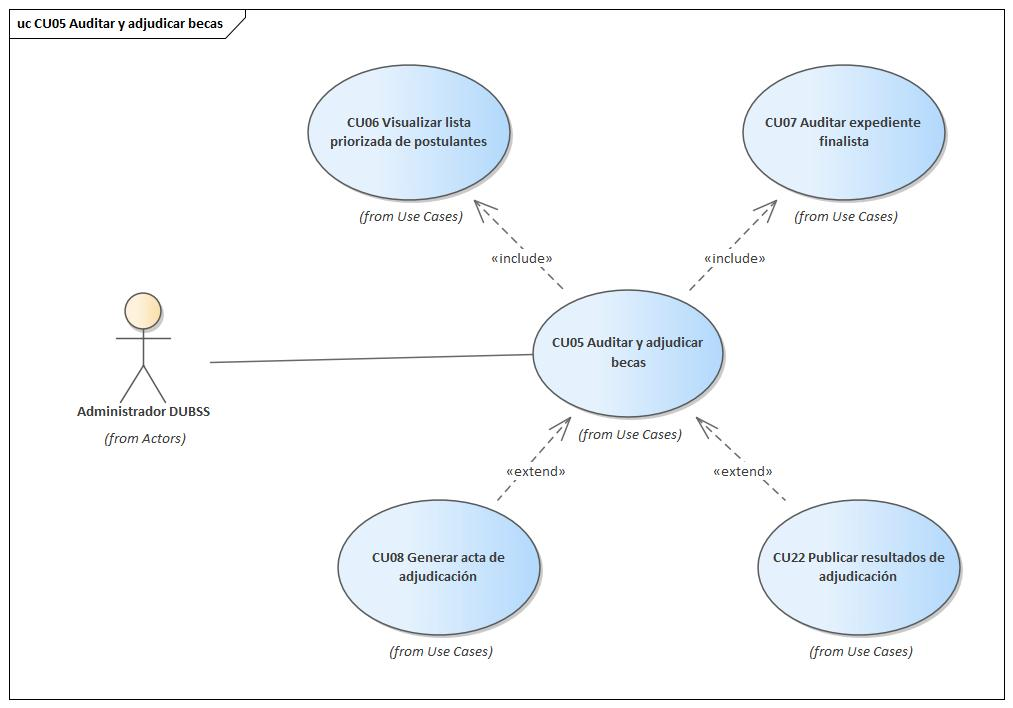
\includegraphics[width=0.8\textwidth,height=0.4\textheight,keepaspectratio]{images/064_CU05_Auditar_Adjudicar_Becas.jpg}

\smallskip
\noindent\raggedright\textit{Nota.} Elaboración propia.
\end{figure}

\refstepcounter{table}\label{tab:detalle_cu05}
\addcontentsline{lot}{table}{\protect\numberline{\thetable}Detalle del CU-05: Auditar y adjudicar becas}
\noindent\textbf{Tabla~\thetable}\par\nopagebreak
\noindent\textit{Detalle del CU-05: Auditar y adjudicar becas}\par\nopagebreak
\begingroup\small\linespread{1}\selectfont
\begin{longtable}{>{\raggedright\arraybackslash}p{2.9cm} >{\raggedright\arraybackslash}p{12.6cm}}
\toprule
\textbf{Caso de Uso} & \textbf{CU-05. Auditar y adjudicar becas} \\
\midrule
\endfirsthead
\toprule
\textbf{Caso de Uso} & \textbf{CU-05. Auditar y adjudicar becas} \\
\midrule
\endhead
\endfoot
\bottomrule
\multicolumn{2}{l}{\textit{Nota.} Elaboración propia.} \\
\endlastfoot
\textbf{Propósito} & Permitir al Administrador DUBSS conducir el proceso de selección de los beneficiarios: identificar a los finalistas mejor puntuados, auditar sus expedientes y registrar la decisión de adjudicar o no adjudicar la Beca Comedor a cada uno de ellos. \\
\midrule
\textbf{Descripción} & Este caso de uso describe el proceso completo de auditoría y adjudicación de una convocatoria. A partir de la lista priorizada por el puntaje de vulnerabilidad (se incluye el CU-06), el Administrador DUBSS selecciona a los finalistas, audita el expediente de cada uno (se incluye el CU-07) y registra la decisión de adjudicación, que queda asociada a la postulación junto con el puntaje vigente, el usuario que decide y la fecha de adjudicación. El CU-08 lo extiende para generar el acta de adjudicación y el CU-22 para publicar los resultados. Respalda el RF-04. \\
\midrule
\textbf{Actores} & Administrador DUBSS. \\
\midrule
\textbf{Actor Iniciador} & Administrador DUBSS. \\
\midrule
\textbf{Precondición} & \vspace{-\baselineskip}\begin{cuvin}
    \item El Administrador DUBSS está autenticado en el sistema (CU-01) con el rol Administrador DUBSS.
    \item La convocatoria de la gestión académica vigente se encuentra cerrada a la recepción de postulaciones (CU-13).
    \item Existen postulaciones en estado «calificada», con puntaje de vulnerabilidad vigente (CU-03).
    \item La convocatoria tiene registrados el número de cupos y el puntaje mínimo requerido (valores por definir con la DUBSS).
\end{cuvin} \\
\midrule
\textbf{Proceso} & \textbf{Flujo principal.}
\begin{cupasos}
    \item El Administrador DUBSS selecciona la opción «Auditoría y adjudicación» y la convocatoria a procesar.
    \item El sistema muestra la lista priorizada de postulantes de la convocatoria (se incluye el CU-06).
    \item El Administrador DUBSS selecciona como finalistas a los postulantes mejor puntuados (cantidad de finalistas por definir con la DUBSS en función de los cupos).
    \item El sistema registra a cada finalista con la posición que ocupa en la lista priorizada.
    \item El Administrador DUBSS audita el expediente de cada finalista (se incluye el CU-07).
    \item El sistema muestra la lista de finalistas con el resultado de su auditoría y el número de cupos disponibles.
    \item El Administrador DUBSS selecciona un finalista auditado y registra su decisión: adjudicar o no adjudicar la beca.
    \item El sistema registra la adjudicación con su resultado, el puntaje vigente de la postulación, el usuario que decide y la fecha de adjudicación.
    \item El sistema actualiza el estado de la postulación a «adjudicada» o «no adjudicada», registra el cambio en el historial de la postulación y en la bitácora, y actualiza el número de cupos disponibles.
    \item Los pasos 7 a 9 se repiten hasta decidir sobre todos los finalistas.
\end{cupasos} \\
 & \textbf{Flujos alternativos.}
\begin{cuvin}
    \item A1 (paso 2): si la convocatoria no tiene postulaciones calificadas, el sistema informa que no existen postulaciones para auditar.
    \item A2 (paso 7): si el expediente del finalista no tiene una auditoría con resultado «validado», el sistema no permite adjudicarle la beca.
    \item A3 (paso 7): si el puntaje de la postulación no alcanza el puntaje mínimo requerido, el sistema no permite adjudicarle la beca.
    \item A4 (paso 7): si los cupos de la convocatoria están agotados, el sistema no permite registrar nuevas adjudicaciones y solo admite la decisión de no adjudicar.
    \item A5 (paso 10): una vez decididas todas las adjudicaciones, el Administrador DUBSS puede generar el acta de adjudicación (CU-08) y publicar los resultados (CU-22).
    \item A6 (paso 7): si los resultados de la convocatoria ya fueron publicados (CU-22), el sistema no permite modificar las adjudicaciones.
    \item A7 (paso 8): si la petición de adjudicación llega duplicada, el sistema la procesa una sola vez (idempotencia).
\end{cuvin} \\
\midrule
\textbf{Postcondición} & \vspace{-\baselineskip}\begin{cuvin}
    \item Cada finalista decidido tiene una adjudicación registrada con su resultado, puntaje final, responsable y fecha de adjudicación.
    \item La postulación queda en estado «adjudicada» o «no adjudicada» y el cambio queda registrado en el historial de la postulación y en la bitácora.
\end{cuvin} \\
\midrule
\textbf{Excepciones} & \vspace{-\baselineskip}\begin{cuvin}
    \item Autenticación inválida o sesión expirada.
    \item Falta de permisos suficientes (el usuario no tiene el rol Administrador DUBSS).
    \item Cupos de la convocatoria agotados.
    \item Error de conexión con el servidor o la base de datos al registrar la adjudicación.
\end{cuvin} \\
\end{longtable}
\endgroup
\addtocounter{table}{-1}

\subsubsection{5.4.6. CU-06 Visualizar lista priorizada de postulantes}\label{sec:cap5_cu06}

\begin{figure}[H]
\caption{Diagrama de contexto del CU-06}
\label{fig:ctx_cu06}
\centering
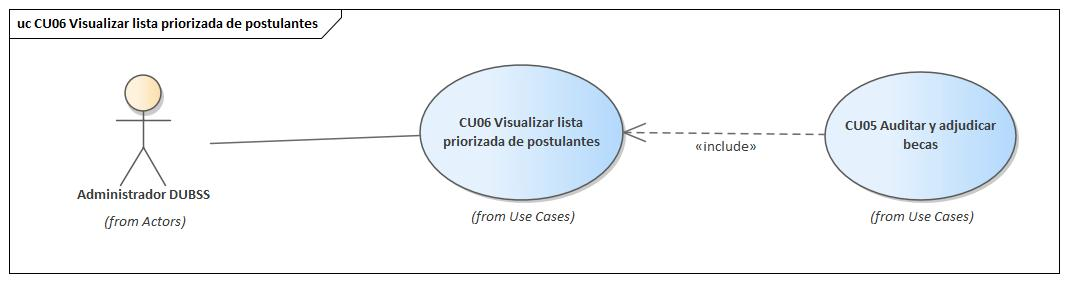
\includegraphics[width=0.8\textwidth,height=0.4\textheight,keepaspectratio]{images/065_CU06_Visualizar_Lista_Priorizada_Postulantes.jpg}

\smallskip
\noindent\raggedright\textit{Nota.} Elaboración propia.
\end{figure}

\refstepcounter{table}\label{tab:detalle_cu06}
\addcontentsline{lot}{table}{\protect\numberline{\thetable}Detalle del CU-06: Visualizar lista priorizada de postulantes}
\noindent\textbf{Tabla~\thetable}\par\nopagebreak
\noindent\textit{Detalle del CU-06: Visualizar lista priorizada de postulantes}\par\nopagebreak
\begingroup\small\linespread{1}\selectfont
\begin{longtable}{>{\raggedright\arraybackslash}p{2.9cm} >{\raggedright\arraybackslash}p{12.6cm}}
\toprule
\textbf{Caso de Uso} & \textbf{CU-06. Visualizar lista priorizada de postulantes} \\
\midrule
\endfirsthead
\toprule
\textbf{Caso de Uso} & \textbf{CU-06. Visualizar lista priorizada de postulantes} \\
\midrule
\endhead
\endfoot
\bottomrule
\multicolumn{2}{l}{\textit{Nota.} Elaboración propia.} \\
\endlastfoot
\textbf{Propósito} & Presentar al Administrador DUBSS las postulaciones de una convocatoria ordenadas de mayor a menor puntaje de vulnerabilidad, para que la auditoría se concentre únicamente en los postulantes mejor puntuados. \\
\midrule
\textbf{Descripción} & Este caso de uso describe cómo el sistema construye y muestra la lista priorizada de postulantes de una convocatoria a partir de las postulaciones en estado «calificada» y de su puntaje vigente calculado por el módulo de IA (CU-03). La lista no se almacena como tal: se obtiene mediante una consulta ordenada y paginada, por lo que siempre refleja el último puntaje calculado. Es incluido por el CU-05. Respalda el RF-04. \\
\midrule
\textbf{Actores} & Administrador DUBSS. \\
\midrule
\textbf{Actor Iniciador} & Administrador DUBSS. \\
\midrule
\textbf{Precondición} & \vspace{-\baselineskip}\begin{cuvin}
    \item El Administrador DUBSS está autenticado en el sistema (CU-01) con el rol Administrador DUBSS.
    \item Existe al menos una convocatoria registrada (CU-13).
    \item Las postulaciones de la convocatoria fueron precalificadas por el módulo de IA (CU-03).
\end{cuvin} \\
\midrule
\textbf{Proceso} & \textbf{Flujo principal.}
\begin{cupasos}
    \item El Administrador DUBSS selecciona la opción «Lista priorizada» (o accede a ella desde el CU-05).
    \item El sistema muestra las convocatorias disponibles.
    \item El Administrador DUBSS selecciona una convocatoria.
    \item El sistema obtiene las postulaciones de la convocatoria en estado «calificada» y su puntaje de vulnerabilidad vigente.
    \item El sistema ordena las postulaciones de mayor a menor puntaje y muestra la lista paginada con: posición, código de postulación, nombre, CI y carrera del postulante, puntaje y fecha de cálculo.
    \item El Administrador DUBSS revisa la lista y, si lo desea, selecciona una postulación para continuar con su auditoría (CU-05).
\end{cupasos} \\
 & \textbf{Flujos alternativos.}
\begin{cuvin}
    \item A1 (paso 4): si la convocatoria no tiene postulaciones calificadas, el sistema muestra un mensaje informativo.
    \item A2 (paso 6): si el Administrador DUBSS aplica un filtro o criterio de ordenamiento (por ejemplo, por carrera), el sistema vuelve a consultar las postulaciones y los puntajes y muestra la lista resultante.
    \item A3 (paso 5): si dos o más postulaciones tienen el mismo puntaje, el sistema aplica el criterio de desempate vigente (por definir con la DUBSS).
    \item A4 (paso 4): las postulaciones en estado «pendiente», «devuelta», «archivada», «adjudicada» o «no adjudicada» no forman parte de la lista priorizada activa; el sistema informa cuántas postulaciones siguen pendientes de precalificación.
\end{cuvin} \\
\midrule
\textbf{Postcondición} & \vspace{-\baselineskip}\begin{cuvin}
    \item El Administrador DUBSS visualiza la lista priorizada de la convocatoria; la consulta no modifica ningún dato del sistema.
\end{cuvin} \\
\midrule
\textbf{Excepciones} & \vspace{-\baselineskip}\begin{cuvin}
    \item Autenticación inválida o sesión expirada.
    \item Falta de permisos suficientes (el usuario no tiene el rol Administrador DUBSS).
    \item Error de conexión con el servidor o la base de datos.
    \item Tiempo de respuesta excedido al consultar un volumen alto de postulaciones (hasta 20,000 por gestión).
\end{cuvin} \\
\end{longtable}
\endgroup
\addtocounter{table}{-1}

\subsubsection{5.4.7. CU-07 Auditar expediente finalista}\label{sec:cap5_cu07}

\begin{figure}[H]
\caption{Diagrama de contexto del CU-07}
\label{fig:ctx_cu07}
\centering
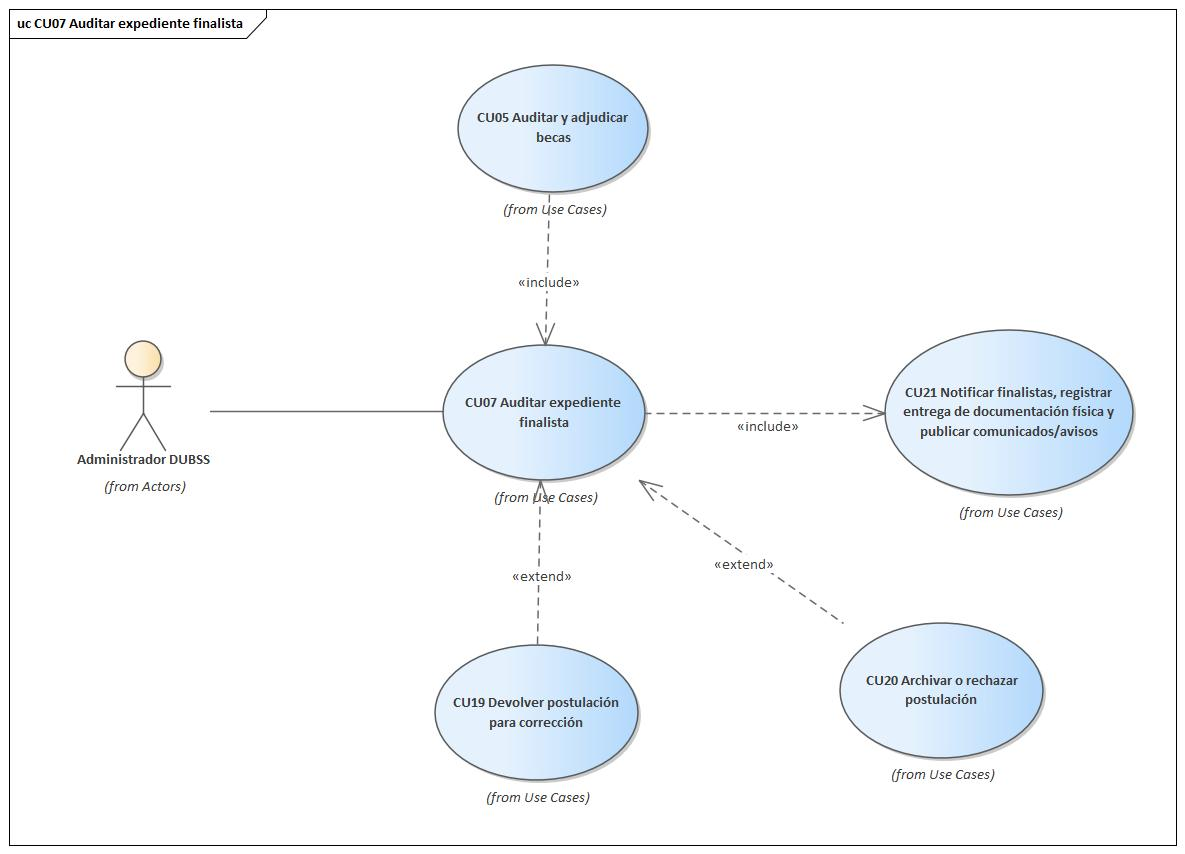
\includegraphics[width=0.8\textwidth,height=0.4\textheight,keepaspectratio]{images/066_CU07_Auditar_Expediente_Finalista.jpg}

\smallskip
\noindent\raggedright\textit{Nota.} Elaboración propia.
\end{figure}

\refstepcounter{table}\label{tab:detalle_cu07}
\addcontentsline{lot}{table}{\protect\numberline{\thetable}Detalle del CU-07: Auditar expediente finalista}
\noindent\textbf{Tabla~\thetable}\par\nopagebreak
\noindent\textit{Detalle del CU-07: Auditar expediente finalista}\par\nopagebreak
\begingroup\small\linespread{1}\selectfont
\begin{longtable}{>{\raggedright\arraybackslash}p{2.9cm} >{\raggedright\arraybackslash}p{12.6cm}}
\toprule
\textbf{Caso de Uso} & \textbf{CU-07. Auditar expediente finalista} \\
\midrule
\endfirsthead
\toprule
\textbf{Caso de Uso} & \textbf{CU-07. Auditar expediente finalista} \\
\midrule
\endhead
\endfoot
\bottomrule
\multicolumn{2}{l}{\textit{Nota.} Elaboración propia.} \\
\endlastfoot
\textbf{Propósito} & Permitir al Administrador DUBSS revisar el expediente de un finalista, cotejar su documentación física con la digital y registrar el resultado de la auditoría. \\
\midrule
\textbf{Descripción} & Este caso de uso describe cómo el Administrador DUBSS audita el expediente de un postulante seleccionado como finalista. El sistema presenta los datos de la postulación, las respuestas socioeconómicas, los documentos digitales adjuntos y el puntaje obtenido; el Administrador coteja esa información con la documentación física entregada por el finalista y registra el resultado de la auditoría (validado, observado o no válido) con sus observaciones. Incluye la notificación al finalista y el registro de la entrega de su documentación física (CU-21). El CU-19 lo extiende para devolver la postulación y el CU-20 para archivarla o rechazarla. Es incluido por el CU-05. Respalda el RF-04. \\
\midrule
\textbf{Actores} & Administrador DUBSS. \\
\midrule
\textbf{Actor Iniciador} & Administrador DUBSS. \\
\midrule
\textbf{Precondición} & \vspace{-\baselineskip}\begin{cuvin}
    \item El Administrador DUBSS está autenticado en el sistema (CU-01) con el rol Administrador DUBSS.
    \item La postulación fue seleccionada como finalista en el CU-05 y se encuentra en estado «calificada».
    \item Los documentos digitales de la postulación están almacenados en Firebase Storage (CU-16).
\end{cuvin} \\
\midrule
\textbf{Proceso} & \textbf{Flujo principal.}
\begin{cupasos}
    \item El Administrador DUBSS selecciona un finalista de la lista de finalistas de la convocatoria.
    \item El sistema muestra el expediente del finalista: datos del postulante, respuestas socioeconómicas, documentos digitales adjuntos, puntaje de vulnerabilidad con su desglose y estado de la entrega de la documentación física.
    \item El sistema notifica al finalista el plazo y los documentos físicos que debe presentar y registra la recepción de dicha documentación (se incluye el CU-21).
    \item El Administrador DUBSS coteja la documentación física entregada con los documentos digitales y los datos declarados.
    \item El Administrador DUBSS registra el resultado de la auditoría (validado, observado o no válido) y sus observaciones.
    \item El sistema registra la auditoría con su resultado, observaciones, auditor y fecha, y deja constancia en la bitácora.
    \item El sistema muestra el expediente como auditado; si el resultado es «validado», el finalista queda habilitado para la decisión de adjudicación (CU-05).
\end{cupasos} \\
 & \textbf{Flujos alternativos.}
\begin{cuvin}
    \item A1 (paso 3): si el finalista no entrega la documentación física dentro del plazo (por definir con la DUBSS), el Administrador DUBSS puede archivar la postulación (CU-20).
    \item A2 (paso 5): si el expediente presenta defectos subsanables, el Administrador DUBSS puede devolver la postulación para su corrección (CU-19).
    \item A3 (paso 5): si la documentación no es válida o la postulación no procede, el Administrador DUBSS puede archivarla o rechazarla (CU-20).
    \item A4 (paso 2): si un documento digital no puede recuperarse de Firebase Storage, el sistema informa el error y permite reintentar la descarga.
    \item A5 (paso 6): si el expediente ya tenía una auditoría (por ejemplo, después de una devolución), el sistema registra la nueva auditoría y conserva las anteriores.
\end{cuvin} \\
\midrule
\textbf{Postcondición} & \vspace{-\baselineskip}\begin{cuvin}
    \item El expediente del finalista tiene registrada una auditoría con su resultado, observaciones, auditor y fecha.
    \item La acción queda registrada en la bitácora.
\end{cuvin} \\
\midrule
\textbf{Excepciones} & \vspace{-\baselineskip}\begin{cuvin}
    \item Autenticación inválida o sesión expirada.
    \item Falta de permisos suficientes (el usuario no tiene el rol Administrador DUBSS).
    \item Error al recuperar los documentos desde Firebase Storage.
    \item Error de conexión con el servidor o la base de datos al registrar la auditoría.
\end{cuvin} \\
\end{longtable}
\endgroup
\addtocounter{table}{-1}

\subsubsection{5.4.8. CU-08 Generar acta de adjudicación}\label{sec:cap5_cu08}

\begin{figure}[H]
\caption{Diagrama de contexto del CU-08}
\label{fig:ctx_cu08}
\centering
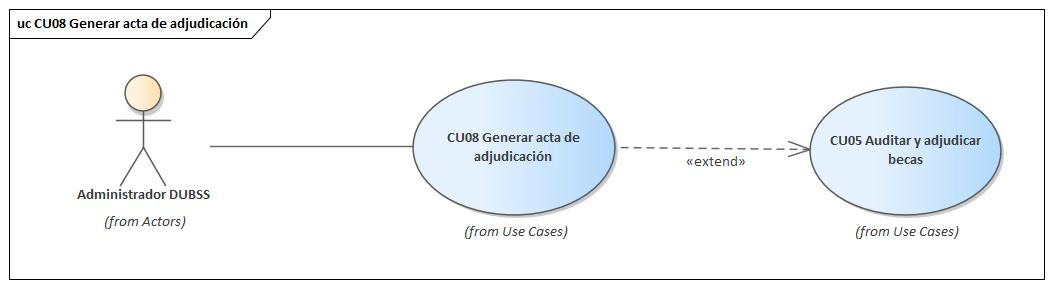
\includegraphics[width=0.8\textwidth,height=0.4\textheight,keepaspectratio]{images/067_CU08_Generar_Acta_Adjudicacion.jpg}

\smallskip
\noindent\raggedright\textit{Nota.} Elaboración propia.
\end{figure}

\refstepcounter{table}\label{tab:detalle_cu08}
\addcontentsline{lot}{table}{\protect\numberline{\thetable}Detalle del CU-08: Generar acta de adjudicación}
\noindent\textbf{Tabla~\thetable}\par\nopagebreak
\noindent\textit{Detalle del CU-08: Generar acta de adjudicación}\par\nopagebreak
\begingroup\small\linespread{1}\selectfont
\begin{longtable}{>{\raggedright\arraybackslash}p{2.9cm} >{\raggedright\arraybackslash}p{12.6cm}}
\toprule
\textbf{Caso de Uso} & \textbf{CU-08. Generar acta de adjudicación} \\
\midrule
\endfirsthead
\toprule
\textbf{Caso de Uso} & \textbf{CU-08. Generar acta de adjudicación} \\
\midrule
\endhead
\endfoot
\bottomrule
\multicolumn{2}{l}{\textit{Nota.} Elaboración propia.} \\
\endlastfoot
\textbf{Propósito} & Generar el acta oficial que deja constancia de los resultados de la adjudicación de la Beca Comedor de una convocatoria. \\
\midrule
\textbf{Descripción} & Este caso de uso describe cómo el Administrador DUBSS genera, una vez decididas todas las adjudicaciones de una convocatoria, el acta de adjudicación en formato PDF con la lista de beneficiarios aprobados. El acta se almacena en Firebase Storage, se registra con un número único y puede consultarse posteriormente. El formato y el contenido oficial del acta están por definir con la DUBSS. Extiende el CU-05. Respalda el RF-04. \\
\midrule
\textbf{Actores} & Administrador DUBSS. \\
\midrule
\textbf{Actor Iniciador} & Administrador DUBSS. \\
\midrule
\textbf{Precondición} & \vspace{-\baselineskip}\begin{cuvin}
    \item El Administrador DUBSS está autenticado en el sistema (CU-01) con el rol Administrador DUBSS.
    \item Todas las adjudicaciones de los finalistas de la convocatoria están decididas (CU-05).
\end{cuvin} \\
\midrule
\textbf{Proceso} & \textbf{Flujo principal A: generar el acta.}
\begin{cupasos}
    \item El Administrador DUBSS selecciona la opción «Generar acta de adjudicación» de la convocatoria.
    \item El sistema verifica que no existan finalistas con la adjudicación pendiente de decisión.
    \item El sistema obtiene las adjudicaciones de la convocatoria con el nombre, CI, carrera y puntaje final de cada postulante adjudicado.
    \item El sistema genera el acta en formato PDF con un número único, la fecha, los datos de la convocatoria y de la gestión académica y la lista de adjudicados.
    \item El sistema almacena el PDF en Firebase Storage y registra el acta con su número, la ruta del archivo, el usuario que la genera y la fecha de generación, y deja constancia en la bitácora.
    \item El sistema muestra el acta generada y permite descargarla e imprimirla.
\end{cupasos} \\
 & \textbf{Flujo principal B: consultar el acta.}
\begin{cupasos}
    \item El Administrador DUBSS selecciona la opción «Consultar acta» de la convocatoria.
    \item El sistema obtiene el acta registrada y la muestra para su descarga e impresión.
\end{cupasos} \\
 & \textbf{Flujos alternativos.}
\begin{cuvin}
    \item A1 (flujo A, paso 2): si existen adjudicaciones pendientes de decisión, el sistema no genera el acta e indica cuántas faltan.
    \item A2 (flujo A, paso 1): si la convocatoria ya tiene un acta generada, el sistema muestra el acta existente en lugar de generar una nueva.
    \item A3 (flujo A, paso 5): si ocurre un error al almacenar el PDF, el sistema no registra el acta y permite reintentar.
    \item A4 (flujo B, paso 2): si la convocatoria aún no tiene un acta generada, el sistema lo informa.
\end{cuvin} \\
\midrule
\textbf{Postcondición} & \vspace{-\baselineskip}\begin{cuvin}
    \item El acta de adjudicación de la convocatoria queda almacenada en Firebase Storage y registrada con su número, responsable y fecha de generación.
    \item La generación del acta queda registrada en la bitácora.
\end{cuvin} \\
\midrule
\textbf{Excepciones} & \vspace{-\baselineskip}\begin{cuvin}
    \item Autenticación inválida o sesión expirada.
    \item Falta de permisos suficientes (el usuario no tiene el rol Administrador DUBSS).
    \item Error al generar el documento PDF.
    \item Error al almacenar el archivo en Firebase Storage.
    \item Error de conexión con el servidor o la base de datos.
\end{cuvin} \\
\end{longtable}
\endgroup
\addtocounter{table}{-1}

\subsubsection{5.4.9. CU-09 Generar planilla de asistencia}\label{sec:cap5_cu09}

\begin{figure}[H]
\caption{Diagrama de contexto del CU-09}
\label{fig:ctx_cu09}
\centering
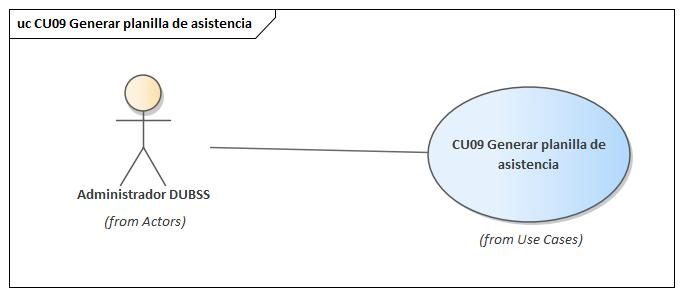
\includegraphics[width=0.8\textwidth,height=0.4\textheight,keepaspectratio]{images/068_CU09_Generar_Planilla_Asistencia.jpg}

\smallskip
\noindent\raggedright\textit{Nota.} Elaboración propia.
\end{figure}

\refstepcounter{table}\label{tab:detalle_cu09}
\addcontentsline{lot}{table}{\protect\numberline{\thetable}Detalle del CU-09: Generar planilla de asistencia}
\noindent\textbf{Tabla~\thetable}\par\nopagebreak
\noindent\textit{Detalle del CU-09: Generar planilla de asistencia}\par\nopagebreak
\begingroup\small\linespread{1}\selectfont
\begin{longtable}{>{\raggedright\arraybackslash}p{2.9cm} >{\raggedright\arraybackslash}p{12.6cm}}
\toprule
\textbf{Caso de Uso} & \textbf{CU-09. Generar planilla de asistencia} \\
\midrule
\endfirsthead
\toprule
\textbf{Caso de Uso} & \textbf{CU-09. Generar planilla de asistencia} \\
\midrule
\endhead
\endfoot
\bottomrule
\multicolumn{2}{l}{\textit{Nota.} Elaboración propia.} \\
\endlastfoot
\textbf{Propósito} & Generar planillas de asistencia imprimibles, a partir del padrón de becados vigente, que sirvan como respaldo físico del uso del beneficio ante las auditorías. \\
\midrule
\textbf{Descripción} & Este caso de uso describe cómo el Administrador DUBSS genera, para un periodo determinado, la planilla de asistencia de los becados vigentes de la convocatoria. La planilla se genera en formato PDF, lista para su impresión, con los espacios para la firma de cada becado y la fotocopia de su carnet, tal como lo exigen las auditorías; se almacena en Firebase Storage y queda disponible para su consulta y para el cotejo con el registro digital (CU-11). Respalda el RF-05. \\
\midrule
\textbf{Actores} & Administrador DUBSS. \\
\midrule
\textbf{Actor Iniciador} & Administrador DUBSS. \\
\midrule
\textbf{Precondición} & \vspace{-\baselineskip}\begin{cuvin}
    \item El Administrador DUBSS está autenticado en el sistema (CU-01) con el rol Administrador DUBSS.
    \item Existe un padrón de becados vigentes para la convocatoria (CU-23).
\end{cuvin} \\
\midrule
\textbf{Proceso} & \textbf{Flujo principal A: generar una planilla.}
\begin{cupasos}
    \item El Administrador DUBSS selecciona la opción «Planillas de asistencia» y la convocatoria correspondiente.
    \item El sistema solicita el periodo de la planilla (fecha desde y fecha hasta).
    \item El Administrador DUBSS ingresa el periodo y confirma la generación.
    \item El sistema valida que la fecha final no sea anterior a la inicial y que el periodo esté comprendido en la gestión académica.
    \item El sistema obtiene las becas en estado vigente de la convocatoria.
    \item El sistema genera la planilla en formato PDF con la lista de becados (nombre, CI y carrera) y los espacios para la firma y la fotocopia del carnet de cada uno (formato por definir con la DUBSS).
    \item El sistema almacena el PDF en Firebase Storage y registra la planilla con su periodo, la ruta del archivo, el usuario que la genera y la fecha de generación.
    \item El sistema muestra la planilla generada para su descarga e impresión.
\end{cupasos} \\
 & \textbf{Flujo principal B: consultar planillas.}
\begin{cupasos}
    \item El Administrador DUBSS selecciona la opción «Consultar planillas» de la convocatoria.
    \item El sistema muestra la lista de planillas generadas con su periodo y fecha de generación, y permite descargar cualquiera de ellas.
\end{cupasos} \\
 & \textbf{Flujos alternativos.}
\begin{cuvin}
    \item A1 (flujo A, paso 4): si el periodo es inválido, el sistema lo indica y permite corregirlo.
    \item A2 (flujo A, paso 5): si la convocatoria no tiene becas vigentes, el sistema no genera la planilla e informa el motivo.
    \item A3 (flujo A, paso 7): si ocurre un error al almacenar el PDF, el sistema no registra la planilla y permite reintentar.
    \item A4 (flujo A, paso 5): la planilla refleja el padrón vigente al momento de su generación; los cambios posteriores en el padrón (CU-23) se reflejan en las planillas que se generen después.
\end{cuvin} \\
\midrule
\textbf{Postcondición} & \vspace{-\baselineskip}\begin{cuvin}
    \item La planilla de asistencia queda almacenada en Firebase Storage y registrada con su periodo, responsable y fecha de generación.
    \item La planilla queda disponible para su impresión y para el cotejo con el registro digital (CU-11).
\end{cuvin} \\
\midrule
\textbf{Excepciones} & \vspace{-\baselineskip}\begin{cuvin}
    \item Autenticación inválida o sesión expirada.
    \item Falta de permisos suficientes (el usuario no tiene el rol Administrador DUBSS).
    \item Error al generar el documento PDF.
    \item Error al almacenar el archivo en Firebase Storage.
    \item Error de conexión con el servidor o la base de datos.
\end{cuvin} \\
\end{longtable}
\endgroup
\addtocounter{table}{-1}

\subsubsection{5.4.10. CU-10 Registrar asistencia digital}\label{sec:cap5_cu10}

\begin{figure}[H]
\caption{Diagrama de contexto del CU-10}
\label{fig:ctx_cu10}
\centering
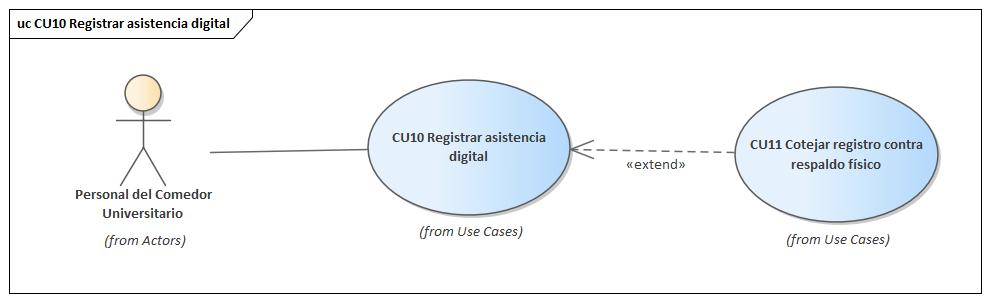
\includegraphics[width=0.8\textwidth,height=0.4\textheight,keepaspectratio]{images/069_CU10_Registrar_Asistencia_Digital.jpg}

\smallskip
\noindent\raggedright\textit{Nota.} Elaboración propia.
\end{figure}

\refstepcounter{table}\label{tab:detalle_cu10}
\addcontentsline{lot}{table}{\protect\numberline{\thetable}Detalle del CU-10: Registrar asistencia digital}
\noindent\textbf{Tabla~\thetable}\par\nopagebreak
\noindent\textit{Detalle del CU-10: Registrar asistencia digital}\par\nopagebreak
\begingroup\small\linespread{1}\selectfont
\begin{longtable}{>{\raggedright\arraybackslash}p{2.9cm} >{\raggedright\arraybackslash}p{12.6cm}}
\toprule
\textbf{Caso de Uso} & \textbf{CU-10. Registrar asistencia digital} \\
\midrule
\endfirsthead
\toprule
\textbf{Caso de Uso} & \textbf{CU-10. Registrar asistencia digital} \\
\midrule
\endhead
\endfoot
\bottomrule
\multicolumn{2}{l}{\textit{Nota.} Elaboración propia.} \\
\endlastfoot
\textbf{Propósito} & Registrar digitalmente la asistencia diaria de cada becado al Comedor Universitario, una vez verificada su identidad por el personal del comedor. \\
\midrule
\textbf{Descripción} & Este caso de uso describe cómo el Personal del Comedor Universitario registra, desde la aplicación móvil, la asistencia diaria de un becado. El sistema no cuenta con un mecanismo biométrico propio: la verificación de identidad la realiza el comedor por sus propios medios y el sistema solo registra su resultado. Se admite un único registro por becado y por día, de modo que las peticiones duplicadas no generan registros adicionales. El CU-11 lo extiende para cotejar el registro digital contra el respaldo físico. Respalda el RF-05. \\
\midrule
\textbf{Actores} & Personal del Comedor Universitario. \\
\midrule
\textbf{Actor Iniciador} & Personal del Comedor Universitario. \\
\midrule
\textbf{Precondición} & \vspace{-\baselineskip}\begin{cuvin}
    \item El Personal del Comedor Universitario está autenticado en la aplicación móvil (CU-01) con el rol Personal del Comedor Universitario.
    \item Existe un padrón de becados vigentes (CU-23).
    \item El personal del comedor verificó la identidad del becado por los medios propios del comedor.
\end{cuvin} \\
\midrule
\textbf{Proceso} & \textbf{Flujo principal.}
\begin{cupasos}
    \item El Personal del Comedor Universitario selecciona la opción «Registrar asistencia» en la aplicación móvil.
    \item El sistema muestra la fecha actual y solicita el CI del becado.
    \item El Personal del Comedor Universitario ingresa el CI del becado.
    \item El sistema busca la beca asociada al CI y verifica que se encuentre en estado vigente.
    \item El sistema muestra los datos del becado: nombre, CI, carrera y estado de la beca.
    \item El Personal del Comedor Universitario confirma el registro de la asistencia.
    \item El sistema verifica que no exista un registro de asistencia de esa beca en la fecha actual.
    \item El sistema registra la asistencia con la fecha, la hora de registro y el usuario que la registra.
    \item El sistema confirma el registro y queda listo para el siguiente becado.
\end{cupasos} \\
 & \textbf{Flujos alternativos.}
\begin{cuvin}
    \item A1 (paso 4): si el CI no corresponde a ningún becado, el sistema informa que el estudiante no figura en el padrón de becados.
    \item A2 (paso 4): si la beca se encuentra suspendida o dada de baja, el sistema no permite el registro e informa el estado de la beca.
    \item A3 (paso 7): si la asistencia del día ya fue registrada, el sistema no crea un nuevo registro e informa la hora del registro existente (idempotencia).
    \item A4 (paso 9): durante una auditoría, el Administrador DUBSS puede cotejar los registros digitales contra la planilla física firmada (CU-11).
\end{cuvin} \\
\midrule
\textbf{Postcondición} & \vspace{-\baselineskip}\begin{cuvin}
    \item La asistencia del becado queda registrada una sola vez para la fecha, con la hora y el usuario que la registró.
    \item El registro queda disponible para la consulta del becado (CU-24), el cotejo (CU-11) y los indicadores de BI (CU-12).
\end{cuvin} \\
\midrule
\textbf{Excepciones} & \vspace{-\baselineskip}\begin{cuvin}
    \item Autenticación inválida o sesión expirada.
    \item Falta de permisos suficientes (el usuario no tiene el rol Personal del Comedor Universitario).
    \item Becado inexistente o beca no vigente.
    \item Error de conexión con el servidor o la base de datos (la asistencia no se registra y debe reintentarse).
\end{cuvin} \\
\end{longtable}
\endgroup
\addtocounter{table}{-1}

\subsubsection{5.4.11. CU-11 Cotejar registro contra respaldo físico}\label{sec:cap5_cu11}

\begin{figure}[H]
\caption{Diagrama de contexto del CU-11}
\label{fig:ctx_cu11}
\centering
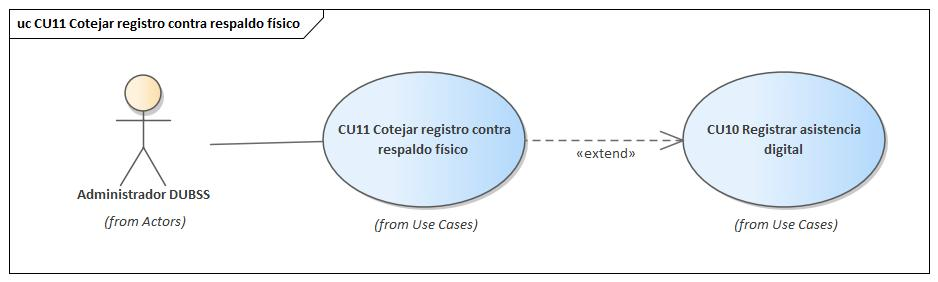
\includegraphics[width=0.8\textwidth,height=0.4\textheight,keepaspectratio]{images/070_CU11_Cotejar_Registro_Respaldo_Fisico.jpg}

\smallskip
\noindent\raggedright\textit{Nota.} Elaboración propia.
\end{figure}

\refstepcounter{table}\label{tab:detalle_cu11}
\addcontentsline{lot}{table}{\protect\numberline{\thetable}Detalle del CU-11: Cotejar registro contra respaldo físico}
\noindent\textbf{Tabla~\thetable}\par\nopagebreak
\noindent\textit{Detalle del CU-11: Cotejar registro contra respaldo físico}\par\nopagebreak
\begingroup\small\linespread{1}\selectfont
\begin{longtable}{>{\raggedright\arraybackslash}p{2.9cm} >{\raggedright\arraybackslash}p{12.6cm}}
\toprule
\textbf{Caso de Uso} & \textbf{CU-11. Cotejar registro contra respaldo físico} \\
\midrule
\endfirsthead
\toprule
\textbf{Caso de Uso} & \textbf{CU-11. Cotejar registro contra respaldo físico} \\
\midrule
\endhead
\endfoot
\bottomrule
\multicolumn{2}{l}{\textit{Nota.} Elaboración propia.} \\
\endlastfoot
\textbf{Propósito} & Permitir al Administrador DUBSS comparar el registro digital de asistencia con la planilla física firmada, para dejar constancia de su coincidencia ante las auditorías. \\
\midrule
\textbf{Descripción} & Este caso de uso describe cómo el Administrador DUBSS, durante una auditoría, selecciona una planilla de asistencia generada (CU-09), consulta los registros digitales de asistencia del mismo periodo (CU-10) y los compara con la planilla física firmada por los becados. El resultado del cotejo (número de registros, coincidencias, discrepancias, observaciones y resultado) queda registrado. El cotejo no modifica los registros de asistencia. Extiende el CU-10. Respalda el RF-05. \\
\midrule
\textbf{Actores} & Administrador DUBSS. \\
\midrule
\textbf{Actor Iniciador} & Administrador DUBSS. \\
\midrule
\textbf{Precondición} & \vspace{-\baselineskip}\begin{cuvin}
    \item El Administrador DUBSS está autenticado en el sistema (CU-01) con el rol Administrador DUBSS.
    \item Existe una planilla de asistencia generada para el periodo a cotejar (CU-09).
    \item El Administrador DUBSS dispone de la planilla física firmada correspondiente.
\end{cuvin} \\
\midrule
\textbf{Proceso} & \textbf{Flujo principal.}
\begin{cupasos}
    \item El Administrador DUBSS selecciona la opción «Cotejo de asistencia» y la planilla a cotejar.
    \item El sistema obtiene la planilla y los registros digitales de asistencia de los becados en el periodo de la planilla.
    \item El sistema muestra, por becado y por día, los registros digitales de asistencia junto con la estructura de la planilla.
    \item El Administrador DUBSS compara los registros digitales con las firmas de la planilla física.
    \item El Administrador DUBSS registra el resultado del cotejo: total de registros, coincidencias, discrepancias, observaciones y resultado (conforme o con discrepancias).
    \item El sistema registra el cotejo con el usuario que lo realiza y la fecha, y deja constancia en la bitácora.
    \item El sistema confirma el registro del cotejo.
\end{cupasos} \\
 & \textbf{Flujos alternativos.}
\begin{cuvin}
    \item A1 (paso 2): si no existen registros digitales en el periodo de la planilla, el sistema lo informa.
    \item A2 (paso 5): si el resultado es «con discrepancias», el sistema exige registrar observaciones.
    \item A3 (paso 6): si la planilla ya fue cotejada, el sistema registra el nuevo cotejo y conserva los anteriores.
\end{cuvin} \\
\midrule
\textbf{Postcondición} & \vspace{-\baselineskip}\begin{cuvin}
    \item El cotejo queda registrado con su resultado, responsable y fecha, y la acción queda en la bitácora.
    \item Los registros de asistencia digital no se modifican.
\end{cuvin} \\
\midrule
\textbf{Excepciones} & \vspace{-\baselineskip}\begin{cuvin}
    \item Autenticación inválida o sesión expirada.
    \item Falta de permisos suficientes (el usuario no tiene el rol Administrador DUBSS).
    \item Datos del cotejo incompletos o inválidos.
    \item Error de conexión con el servidor o la base de datos.
\end{cuvin} \\
\end{longtable}
\endgroup
\addtocounter{table}{-1}

\subsubsection{5.4.12. CU-12 Visualizar dashboard de indicadores BI}\label{sec:cap5_cu12}

\begin{figure}[H]
\caption{Diagrama de contexto del CU-12}
\label{fig:ctx_cu12}
\centering
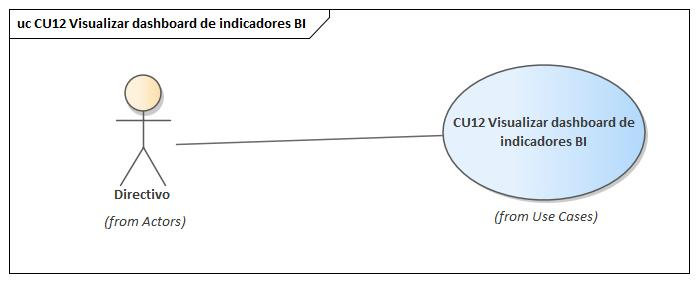
\includegraphics[width=0.8\textwidth,height=0.4\textheight,keepaspectratio]{images/071_CU12_Visualizar_Dashboard_Indicadores_BI.jpg}

\smallskip
\noindent\raggedright\textit{Nota.} Elaboración propia.
\end{figure}

\refstepcounter{table}\label{tab:detalle_cu12}
\addcontentsline{lot}{table}{\protect\numberline{\thetable}Detalle del CU-12: Visualizar dashboard de indicadores BI}
\noindent\textbf{Tabla~\thetable}\par\nopagebreak
\noindent\textit{Detalle del CU-12: Visualizar dashboard de indicadores BI}\par\nopagebreak
\begingroup\small\linespread{1}\selectfont
\begin{longtable}{>{\raggedright\arraybackslash}p{2.9cm} >{\raggedright\arraybackslash}p{12.6cm}}
\toprule
\textbf{Caso de Uso} & \textbf{CU-12. Visualizar dashboard de indicadores BI} \\
\midrule
\endfirsthead
\toprule
\textbf{Caso de Uso} & \textbf{CU-12. Visualizar dashboard de indicadores BI} \\
\midrule
\endhead
\endfoot
\bottomrule
\multicolumn{2}{l}{\textit{Nota.} Elaboración propia.} \\
\endlastfoot
\textbf{Propósito} & Brindar al Directivo un dashboard interactivo de Business Intelligence con los indicadores clave del proceso de la Beca Comedor, como apoyo a la toma de decisiones. \\
\midrule
\textbf{Descripción} & Este caso de uso describe cómo el Directivo consulta el dashboard de indicadores: postulaciones recibidas, finalistas, becas adjudicadas y asistencia, por convocatoria y por mes, con la posibilidad de filtrarlos por gestión académica. Los indicadores se obtienen de vistas precalculadas que se actualizan por lotes, de modo que la consulta no afecta el rendimiento de las operaciones transaccionales. Es una consulta de solo lectura. Respalda el RF-07. \\
\midrule
\textbf{Actores} & Directivo. \\
\midrule
\textbf{Actor Iniciador} & Directivo. \\
\midrule
\textbf{Precondición} & \vspace{-\baselineskip}\begin{cuvin}
    \item El Directivo está autenticado en el sistema (CU-01) con el rol Directivo.
    \item Los indicadores fueron calculados en el último proceso por lotes.
\end{cuvin} \\
\midrule
\textbf{Proceso} & \textbf{Flujo principal.}
\begin{cupasos}
    \item El Directivo selecciona la opción «Dashboard de indicadores».
    \item El sistema consulta los indicadores precalculados de la gestión académica vigente.
    \item El sistema muestra en gráficos interactivos los indicadores de postulaciones recibidas, finalistas, becas adjudicadas y asistencia, por convocatoria y por mes, junto con la fecha de su última actualización.
    \item El Directivo selecciona una gestión académica para filtrar los indicadores.
    \item El sistema consulta los indicadores de la gestión seleccionada y actualiza el dashboard.
\end{cupasos} \\
 & \textbf{Flujos alternativos.}
\begin{cuvin}
    \item A1 (pasos 2 y 5): si no existen datos para la gestión académica consultada, el sistema muestra un mensaje informativo.
    \item A2 (paso 3): si el proceso por lotes aún no se ha ejecutado, el sistema muestra los últimos indicadores disponibles con su fecha de actualización.
\end{cuvin} \\
\midrule
\textbf{Postcondición} & \vspace{-\baselineskip}\begin{cuvin}
    \item El Directivo visualiza los indicadores; la consulta no modifica ningún dato del sistema.
\end{cuvin} \\
\midrule
\textbf{Excepciones} & \vspace{-\baselineskip}\begin{cuvin}
    \item Autenticación inválida o sesión expirada.
    \item Falta de permisos suficientes (el usuario no tiene el rol Directivo).
    \item Error de conexión con el servidor o la base de datos.
\end{cuvin} \\
\end{longtable}
\endgroup
\addtocounter{table}{-1}

\subsubsection{5.4.13. CU-13 Gestionar convocatoria y gestión académica}\label{sec:cap5_cu13}

\begin{figure}[H]
\caption{Diagrama de contexto del CU-13}
\label{fig:ctx_cu13}
\centering
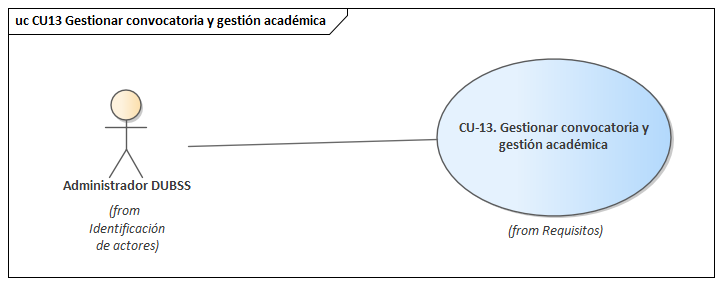
\includegraphics[width=0.8\textwidth,height=0.4\textheight,keepaspectratio]{images/042_CU13_Gestionar_Convocatoria_Gestion_Academica.png}

\smallskip
\noindent\raggedright\textit{Nota.} Elaboración propia.
\end{figure}

\refstepcounter{table}\label{tab:detalle_cu13}
\addcontentsline{lot}{table}{\protect\numberline{\thetable}Detalle del CU-13: Gestionar convocatoria y gestión académica}
\noindent\textbf{Tabla~\thetable}\par\nopagebreak
\noindent\textit{Detalle del CU-13: Gestionar convocatoria y gestión académica}\par\nopagebreak
\begingroup\small\linespread{1}\selectfont
\begin{longtable}{>{\raggedright\arraybackslash}p{2.9cm} >{\raggedright\arraybackslash}p{12.6cm}}
\toprule
\textbf{Caso de Uso} & \textbf{CU-13. Gestionar convocatoria y gestión académica} \\
\midrule
\endfirsthead
\toprule
\textbf{Caso de Uso} & \textbf{CU-13. Gestionar convocatoria y gestión académica} \\
\midrule
\endhead
\endfoot
\bottomrule
\multicolumn{2}{l}{\textit{Nota.} Elaboración propia.} \\
\endlastfoot
\textbf{Propósito} & Permitir al Administrador DUBSS crear, editar, abrir y cerrar las convocatorias de la Beca Comedor, controlando el periodo en que se reciben postulaciones. \\
\midrule
\textbf{Descripción} & Este caso de uso describe cómo el Administrador DUBSS gestiona las convocatorias y las gestiones académicas, definiendo las fechas de apertura y cierre, el número de cupos y la lista de documentos obligatorios. Solo puede recibirse una postulación (CU-02) mientras la convocatoria esté abierta, y cada postulación queda asociada a la gestión vigente. Respalda el RF-08. \\
\midrule
\textbf{Actores} & Administrador DUBSS. \\
\midrule
\textbf{Actor Iniciador} & Administrador DUBSS. \\
\midrule
\textbf{Precondición} & \vspace{-\baselineskip}\begin{cuvin}
    \item El Administrador DUBSS está autenticado en el sistema (CU-01).
    \item El Administrador cuenta con privilegios de administración.
\end{cuvin} \\
\midrule
\textbf{Proceso} & \textbf{Flujo principal.}
\begin{cupasos}
    \item El Administrador accede a la opción «Convocatorias».
    \item El sistema muestra la lista de convocatorias con su gestión académica, fechas, cupos y estado (programada, abierta o cerrada).
    \item El Administrador selecciona la acción deseada: crear, editar, abrir, cerrar o consultar una convocatoria.
    \item Para crear o editar, el Administrador ingresa la gestión académica, la fecha de apertura, la fecha de cierre, el número de cupos (por definir con la DUBSS) y la lista de documentos obligatorios (nombre, tipo y formatos permitidos).
    \item El sistema valida que la fecha de cierre sea posterior a la de apertura, que no exista otra convocatoria vigente para la misma gestión académica y que se haya definido al menos un documento obligatorio.
    \item El Administrador confirma la operación.
    \item El sistema guarda la convocatoria, actualiza su estado y registra la acción en la bitácora (CU-25).
    \item El sistema confirma la operación y muestra la lista actualizada.
\end{cupasos} \\
 & \textbf{Flujos alternativos.}
\begin{cuvin}
    \item A1 (paso 5): si ya existe una convocatoria vigente para la misma gestión académica, el sistema rechaza la operación e informa del conflicto.
    \item A2 (paso 5): si las fechas son incoherentes (cierre anterior o igual a la apertura) o hay datos obligatorios vacíos, el sistema indica los errores y permite corregirlos.
    \item A3 (paso 3): al abrir una convocatoria, el sistema cambia su estado a «abierta» y habilita el envío de postulaciones desde esa fecha.
    \item A4 (paso 3): al cerrar una convocatoria, el sistema cambia su estado a «cerrada», bloquea el envío de nuevas postulaciones y descarta o bloquea los borradores no enviados (CU-17).
    \item A5 (paso 3): si la fecha de cierre se cumple, el sistema cierra la convocatoria automáticamente.
    \item A6 (paso 4): si la convocatoria ya tiene postulaciones recibidas, el sistema restringe la edición de los documentos obligatorios y de las fechas de apertura (alcance por definir con la DUBSS) para no afectar las postulaciones existentes.
    \item A7 (paso 3): el sistema no permite eliminar una convocatoria con postulaciones asociadas; solo permite cerrarla.
\end{cuvin} \\
\midrule
\textbf{Postcondición} & \vspace{-\baselineskip}\begin{cuvin}
    \item La convocatoria queda registrada o actualizada con su gestión, fechas, cupos y documentos requeridos.
    \item El estado de la convocatoria determina si el sistema acepta o no nuevas postulaciones.
    \item La operación queda registrada en la bitácora.
\end{cuvin} \\
\midrule
\textbf{Excepciones} & \vspace{-\baselineskip}\begin{cuvin}
    \item Autenticación inválida o sesión expirada.
    \item Falta de permisos suficientes (el usuario no tiene el rol Administrador DUBSS).
    \item Datos ingresados no válidos o convocatoria duplicada para la gestión.
    \item Intento de eliminar una convocatoria con postulaciones asociadas.
    \item Error de conexión con el servidor o la base de datos.
\end{cuvin} \\
\end{longtable}
\endgroup
\addtocounter{table}{-1}

\subsubsection{5.4.14. CU-14 Gestionar usuarios y roles}\label{sec:cap5_cu14}

\begin{figure}[H]
\caption{Diagrama de contexto del CU-14}
\label{fig:ctx_cu14}
\centering
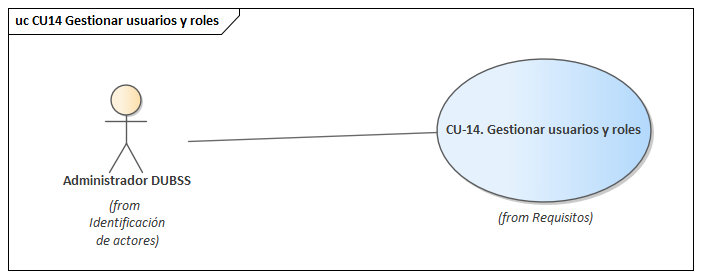
\includegraphics[width=0.8\textwidth,height=0.4\textheight,keepaspectratio]{images/043_CU14_Gestionar_Usuarios_Roles.png}

\smallskip
\noindent\raggedright\textit{Nota.} Elaboración propia.
\end{figure}

\refstepcounter{table}\label{tab:detalle_cu14}
\addcontentsline{lot}{table}{\protect\numberline{\thetable}Detalle del CU-14: Gestionar usuarios y roles}
\noindent\textbf{Tabla~\thetable}\par\nopagebreak
\noindent\textit{Detalle del CU-14: Gestionar usuarios y roles}\par\nopagebreak
\begingroup\small\linespread{1}\selectfont
\begin{longtable}{>{\raggedright\arraybackslash}p{2.9cm} >{\raggedright\arraybackslash}p{12.6cm}}
\toprule
\textbf{Caso de Uso} & \textbf{CU-14. Gestionar usuarios y roles} \\
\midrule
\endfirsthead
\toprule
\textbf{Caso de Uso} & \textbf{CU-14. Gestionar usuarios y roles} \\
\midrule
\endhead
\endfoot
\bottomrule
\multicolumn{2}{l}{\textit{Nota.} Elaboración propia.} \\
\endlastfoot
\textbf{Propósito} & Permitir al Administrador DUBSS gestionar las cuentas del personal y asignarles roles, de modo que cada persona acceda únicamente a las funciones que le corresponden. \\
\midrule
\textbf{Descripción} & Este caso de uso describe cómo el Administrador DUBSS crea, edita, desactiva y reactiva las cuentas del personal y les asigna uno de los roles del sistema (Administrador, Directivo o Personal del Comedor). Los Postulantes no se gestionan aquí, pues se registran por sí mismos (CU-01). Las cuentas se crean en la base de datos y los cambios de rol se conservan en la bitácora (CU-25). Respalda el RF-09. \\
\midrule
\textbf{Actores} & Administrador DUBSS. \\
\midrule
\textbf{Actor Iniciador} & Administrador DUBSS. \\
\midrule
\textbf{Precondición} & \vspace{-\baselineskip}\begin{cuvin}
    \item El Administrador DUBSS está autenticado en el sistema (CU-01).
    \item El Administrador cuenta con privilegios de administración.
\end{cuvin} \\
\midrule
\textbf{Proceso} & \textbf{Flujo principal.}
\begin{cupasos}
    \item El Administrador accede a la opción «Usuarios y roles».
    \item El sistema muestra la lista de cuentas del personal con su nombre, CI, correo, rol y estado (activa o desactivada), con filtros por rol, estado y búsqueda por CI o nombre.
    \item El Administrador selecciona la acción deseada: crear, editar, cambiar rol, desactivar o reactivar una cuenta.
    \item Para crear una cuenta, el Administrador ingresa los datos del funcionario (nombres, apellidos, CI, correo electrónico y rol).
    \item El sistema valida que los datos sean correctos y que el CI y el correo electrónico no estén registrados.
    \item El Administrador confirma la operación.
    \item El sistema crea o actualiza la cuenta en la base de datos y genera una contraseña temporal (o un enlace de activación) para que el usuario establezca su contraseña de acceso.
    \item El sistema registra la acción (usuario, cambio realizado, fecha y hora) en la bitácora y muestra la lista actualizada.
\end{cupasos} \\
 & \textbf{Flujos alternativos.}
\begin{cuvin}
    \item A1 (paso 5): si el CI o el correo electrónico ya están registrados, el sistema rechaza el alta e indica el campo en conflicto.
    \item A2 (paso 5): si faltan datos obligatorios o su formato es inválido, el sistema marca los errores y permite corregirlos.
    \item A3 (paso 3): si se cambia el rol de una cuenta, el sistema aplica los nuevos permisos desde su siguiente inicio de sesión y conserva el registro del cambio (rol anterior, rol nuevo, fecha y responsable).
    \item A4 (paso 3): al desactivar una cuenta, el sistema impide su acceso e invalida sus sesiones activas; la cuenta no se elimina, de modo que se preserve la trazabilidad de sus acciones.
    \item A5 (paso 3): el sistema impide que el Administrador desactive su propia cuenta o la del último Administrador activo.
    \item A6 (paso 3): el Administrador puede reactivar una cuenta desactivada, que recupera su rol anterior.
\end{cuvin} \\
\midrule
\textbf{Postcondición} & \vspace{-\baselineskip}\begin{cuvin}
    \item La cuenta queda creada, modificada, desactivada o reactivada, y el sistema refleja el cambio de rol en los permisos del usuario.
    \item El cambio queda registrado en la bitácora.
\end{cuvin} \\
\midrule
\textbf{Excepciones} & \vspace{-\baselineskip}\begin{cuvin}
    \item Autenticación inválida o sesión expirada.
    \item Falta de permisos suficientes (el usuario no tiene el rol Administrador DUBSS).
    \item Datos ingresados no válidos o CI/correo duplicados.
    \item Error de conexión con el servidor o la base de datos.
\end{cuvin} \\
\end{longtable}
\endgroup
\addtocounter{table}{-1}

\subsubsection{5.4.15. CU-15 Recuperar contraseña / gestionar perfil}\label{sec:cap5_cu15}

\begin{figure}[H]
\caption{Diagrama de contexto del CU-15}
\label{fig:ctx_cu15}
\centering
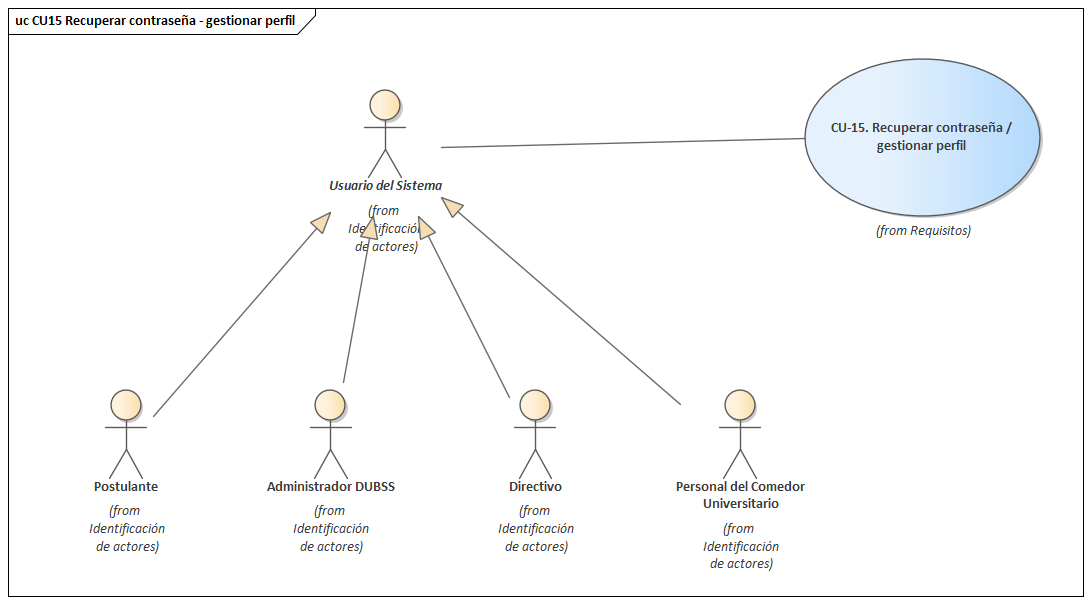
\includegraphics[width=0.8\textwidth,height=0.4\textheight,keepaspectratio]{images/044_CU15_Recuperar_Contrasena_Gestionar_Perfil.png}

\smallskip
\noindent\raggedright\textit{Nota.} Elaboración propia.
\end{figure}

\refstepcounter{table}\label{tab:detalle_cu15}
\addcontentsline{lot}{table}{\protect\numberline{\thetable}Detalle del CU-15: Recuperar contraseña / gestionar perfil}
\noindent\textbf{Tabla~\thetable}\par\nopagebreak
\noindent\textit{Detalle del CU-15: Recuperar contraseña / gestionar perfil}\par\nopagebreak
\begingroup\small\linespread{1}\selectfont
\begin{longtable}{>{\raggedright\arraybackslash}p{2.9cm} >{\raggedright\arraybackslash}p{12.6cm}}
\toprule
\textbf{Caso de Uso} & \textbf{CU-15. Recuperar contraseña / gestionar perfil} \\
\midrule
\endfirsthead
\toprule
\textbf{Caso de Uso} & \textbf{CU-15. Recuperar contraseña / gestionar perfil} \\
\midrule
\endhead
\endfoot
\bottomrule
\multicolumn{2}{l}{\textit{Nota.} Elaboración propia.} \\
\endlastfoot
\textbf{Propósito} & Permitir a los usuarios recuperar el acceso a su cuenta cuando olvidan su contraseña y mantener actualizados sus datos de contacto y su contraseña desde su perfil. \\
\midrule
\textbf{Descripción} & Este caso de uso describe dos funciones: la recuperación de contraseña mediante un enlace enviado al correo registrado (generado por el backend) y la gestión del perfil, donde el usuario autenticado actualiza sus datos de contacto y su contraseña. El CI no puede modificarse desde el perfil. Extiende al CU-01. Respalda el RF-10. \\
\midrule
\textbf{Actores} & Usuario del Sistema (Postulante, Administrador DUBSS, Directivo, Personal del Comedor Universitario). \\
\midrule
\textbf{Actor Iniciador} & Usuario del Sistema. \\
\midrule
\textbf{Precondición} & \vspace{-\baselineskip}\begin{cuvin}
    \item Recuperar contraseña: el usuario tiene una cuenta registrada con un correo electrónico al que puede acceder.
    \item Gestionar perfil: el usuario está autenticado en el sistema (CU-01).
\end{cuvin} \\
\midrule
\textbf{Proceso} & \textbf{Flujo principal A: recuperar contraseña.}
\begin{cupasos}
    \item En la pantalla de inicio de sesión, el usuario selecciona «¿Olvidó su contraseña?».
    \item El sistema solicita el correo electrónico de la cuenta.
    \item El usuario ingresa su correo y confirma la solicitud.
    \item El sistema genera un token de restablecimiento de un solo uso con tiempo de validez limitado, lo envía en un enlace al correo registrado y muestra un mensaje informando que, si el correo está registrado, recibirá las instrucciones.
    \item El usuario abre el enlace recibido y define una nueva contraseña que cumpla la política de seguridad.
    \item El sistema confirma el cambio y permite al usuario iniciar sesión con la nueva contraseña.
\end{cupasos} \\
 & \textbf{Flujo principal B: gestionar perfil.}
\begin{cupasos}
    \item El usuario autenticado accede a la opción «Mi perfil».
    \item El sistema muestra sus datos personales y de contacto; el CI se muestra solo de lectura.
    \item El usuario modifica sus datos de contacto (por ejemplo, correo electrónico y teléfono; campos exactos por definir) y/o solicita cambiar su contraseña ingresando la contraseña actual y la nueva.
    \item El sistema valida los datos, comprueba la unicidad del correo y la política de contraseña.
    \item El sistema guarda los cambios y confirma la actualización.
\end{cupasos} \\
 & \textbf{Flujos alternativos.}
\begin{cuvin}
    \item A1 (flujo A, paso 4): si el correo no está registrado, el sistema muestra el mismo mensaje neutro, para no revelar qué correos existen en el sistema.
    \item A2 (flujo A, paso 5): si el enlace expiró o ya fue utilizado, el sistema informa del hecho y permite solicitar uno nuevo.
    \item A3 (flujo A, paso 5): si la nueva contraseña no cumple la política de seguridad, el sistema muestra los requisitos y permite reintentar.
    \item A4 (flujo B, paso 3): si el usuario intenta modificar su CI, el sistema no lo permite (campo bloqueado).
    \item A5 (flujo B, paso 4): si el nuevo correo electrónico ya pertenece a otra cuenta, el sistema rechaza el cambio.
    \item A6 (flujo B, paso 4): si la contraseña actual ingresada es incorrecta, el sistema rechaza el cambio de contraseña.
    \item A7 (flujo B, paso 5): si se cambia el correo electrónico, el sistema puede requerir una reautenticación previa (criterio por definir).
\end{cuvin} \\
\midrule
\textbf{Postcondición} & \vspace{-\baselineskip}\begin{cuvin}
    \item Recuperar contraseña: la cuenta queda con una nueva contraseña y el usuario puede autenticarse.
    \item Gestionar perfil: los datos de contacto y/o la contraseña quedan actualizados y se utilizarán en las notificaciones al usuario.
\end{cuvin} \\
\midrule
\textbf{Excepciones} & \vspace{-\baselineskip}\begin{cuvin}
    \item Autenticación inválida o sesión expirada (en la gestión de perfil).
    \item Datos ingresados no válidos.
    \item Enlace de restablecimiento inválido o expirado.
    \item Servicio de envío de correo electrónico no disponible.
    \item Error de conexión con el servidor o la base de datos.
\end{cuvin} \\
\end{longtable}
\endgroup
\addtocounter{table}{-1}

\subsubsection{5.4.16. CU-16 Digitalizar y adjuntar documentos}\label{sec:cap5_cu16}

\begin{figure}[H]
\caption{Diagrama de contexto del CU-16}
\label{fig:ctx_cu16}
\centering
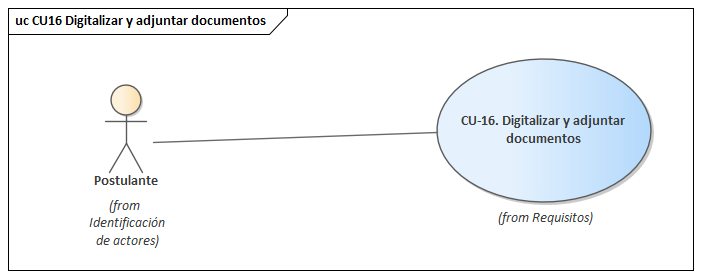
\includegraphics[width=0.8\textwidth,height=0.4\textheight,keepaspectratio]{images/045_CU16_Digitalizar_Adjuntar_Documentos.png}

\smallskip
\noindent\raggedright\textit{Nota.} Elaboración propia.
\end{figure}

\refstepcounter{table}\label{tab:detalle_cu16}
\addcontentsline{lot}{table}{\protect\numberline{\thetable}Detalle del CU-16: Digitalizar y adjuntar documentos}
\noindent\textbf{Tabla~\thetable}\par\nopagebreak
\noindent\textit{Detalle del CU-16: Digitalizar y adjuntar documentos}\par\nopagebreak
\begingroup\small\linespread{1}\selectfont
\begin{longtable}{>{\raggedright\arraybackslash}p{2.9cm} >{\raggedright\arraybackslash}p{12.6cm}}
\toprule
\textbf{Caso de Uso} & \textbf{CU-16. Digitalizar y adjuntar documentos} \\
\midrule
\endfirsthead
\toprule
\textbf{Caso de Uso} & \textbf{CU-16. Digitalizar y adjuntar documentos} \\
\midrule
\endhead
\endfoot
\bottomrule
\multicolumn{2}{l}{\textit{Nota.} Elaboración propia.} \\
\endlastfoot
\textbf{Propósito} & Permitir al Postulante digitalizar sus documentos con la cámara del teléfono, o cargarlos desde un archivo en la web, y asociarlos a su postulación como respaldo de los datos declarados. \\
\midrule
\textbf{Descripción} & Este caso de uso describe cómo el Postulante captura o adjunta cada documento requerido por la convocatoria, valida su formato y tamaño, revisa una vista previa y lo asocia a su postulación, almacenándolo en Firebase Storage. Es incluido por el CU-02 y también se utiliza al completar un borrador (CU-17). Permite evitar la presentación de carpetas físicas en la etapa inicial. Respalda el RF-11. \\
\midrule
\textbf{Actores} & Postulante. \\
\midrule
\textbf{Actor Iniciador} & Postulante. \\
\midrule
\textbf{Precondición} & \vspace{-\baselineskip}\begin{cuvin}
    \item El Postulante está autenticado en el sistema (CU-01).
    \item El Postulante se encuentra completando una postulación o un borrador, con la convocatoria abierta.
    \item La convocatoria tiene definida la lista de documentos requeridos.
    \item En la aplicación móvil, el Postulante otorgó el permiso de uso de la cámara.
\end{cuvin} \\
\midrule
\textbf{Proceso} & \textbf{Flujo principal.}
\begin{cupasos}
    \item El sistema muestra la lista de documentos requeridos por la convocatoria, indicando cuáles están pendientes y cuáles ya fueron adjuntados.
    \item El Postulante selecciona el documento que desea adjuntar.
    \item En la aplicación móvil, el Postulante captura el documento con la cámara del dispositivo; en el portal web, selecciona un archivo de su equipo.
    \item El sistema valida el formato y el tamaño del archivo (formatos y tamaño máximo por definir con la DUBSS).
    \item El sistema muestra una vista previa del documento.
    \item El Postulante confirma el documento, o bien lo reemplaza, lo vuelve a capturar o lo elimina.
    \item El sistema almacena el archivo en Firebase Storage y registra el documento adjunto (tipo y archivo) asociado a la postulación.
    \item El sistema actualiza la lista de documentos con el estado «adjuntado».
\end{cupasos} \\
 & \textbf{Flujos alternativos.}
\begin{cuvin}
    \item A1 (paso 3): si el Postulante no otorga el permiso de la cámara, el sistema le ofrece seleccionar el documento desde la galería o los archivos del dispositivo.
    \item A2 (paso 4): si el formato no es permitido o el tamaño excede el máximo, el sistema rechaza el archivo y muestra un mensaje de error.
    \item A3 (paso 6): el Postulante puede reemplazar o eliminar un documento ya adjuntado, siempre que la postulación no haya sido enviada o se encuentre devuelta (CU-19).
    \item A4 (paso 7): si falla la carga por problemas de conexión, el sistema permite reintentar sin perder los demás documentos ya adjuntados.
    \item A5 (paso 3): el Postulante puede adjuntar más de un archivo o página para un mismo documento (cantidad máxima por definir).
    \item A6 (general): si al enviar la postulación faltan documentos obligatorios, el CU-02 no permite el envío e indica los documentos faltantes.
\end{cuvin} \\
\midrule
\textbf{Postcondición} & \vspace{-\baselineskip}\begin{cuvin}
    \item Los documentos adjuntados quedan almacenados en Firebase Storage y vinculados a la postulación (o al borrador).
    \item La lista de documentos requeridos refleja cuáles fueron cargados y cuáles faltan.
\end{cuvin} \\
\midrule
\textbf{Excepciones} & \vspace{-\baselineskip}\begin{cuvin}
    \item Autenticación inválida o sesión expirada.
    \item Permiso de cámara denegado.
    \item Formato o tamaño de archivo no permitido.
    \item Error al almacenar el archivo en Firebase Storage.
    \item Convocatoria cerrada durante la carga de documentos.
    \item Error de conexión con el servidor.
\end{cuvin} \\
\end{longtable}
\endgroup
\addtocounter{table}{-1}

\subsubsection{5.4.17. CU-17 Guardar borrador de postulación}\label{sec:cap5_cu17}

\begin{figure}[H]
\caption{Diagrama de contexto del CU-17}
\label{fig:ctx_cu17}
\centering
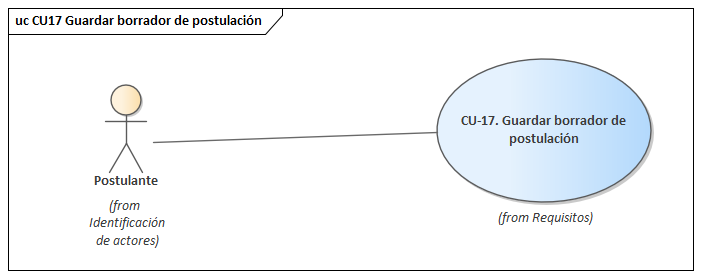
\includegraphics[width=0.8\textwidth,height=0.4\textheight,keepaspectratio]{images/046_CU17_Guardar_Borrador_Postulacion.png}

\smallskip
\noindent\raggedright\textit{Nota.} Elaboración propia.
\end{figure}

\refstepcounter{table}\label{tab:detalle_cu17}
\addcontentsline{lot}{table}{\protect\numberline{\thetable}Detalle del CU-17: Guardar borrador de postulación}
\noindent\textbf{Tabla~\thetable}\par\nopagebreak
\noindent\textit{Detalle del CU-17: Guardar borrador de postulación}\par\nopagebreak
\begingroup\small\linespread{1}\selectfont
\begin{longtable}{>{\raggedright\arraybackslash}p{2.9cm} >{\raggedright\arraybackslash}p{12.6cm}}
\toprule
\textbf{Caso de Uso} & \textbf{CU-17. Guardar borrador de postulación} \\
\midrule
\endfirsthead
\toprule
\textbf{Caso de Uso} & \textbf{CU-17. Guardar borrador de postulación} \\
\midrule
\endhead
\endfoot
\bottomrule
\multicolumn{2}{l}{\textit{Nota.} Elaboración propia.} \\
\endlastfoot
\textbf{Propósito} & Permitir al Postulante guardar su postulación incompleta como borrador y retomarla posteriormente sin perder lo ya ingresado. \\
\midrule
\textbf{Descripción} & Este caso de uso describe cómo el Postulante guarda el avance del formulario socioeconómico y de los documentos adjuntos, sin necesidad de completar los campos obligatorios, y cómo lo retoma después para completarlo y enviarlo. Un borrador no es una postulación enviada, por lo que no se procesa con el módulo de IA ni cuenta como postulación vigente. Extiende al CU-02. Respalda el RF-12. \\
\midrule
\textbf{Actores} & Postulante. \\
\midrule
\textbf{Actor Iniciador} & Postulante. \\
\midrule
\textbf{Precondición} & \vspace{-\baselineskip}\begin{cuvin}
    \item El Postulante está autenticado en el sistema (CU-01).
    \item Existe una convocatoria abierta (CU-13).
    \item El Postulante no tiene una postulación vigente ya enviada en la misma gestión.
\end{cuvin} \\
\midrule
\textbf{Proceso} & \textbf{Flujo principal A: guardar borrador.}
\begin{cupasos}
    \item Durante el llenado del formulario (CU-02), el Postulante selecciona «Guardar borrador».
    \item El sistema verifica que la convocatoria continúe abierta.
    \item El sistema guarda los datos ingresados hasta ese momento y las referencias a los documentos ya adjuntados, sin exigir los campos ni documentos obligatorios.
    \item El sistema registra la fecha y hora del último guardado.
    \item El sistema confirma que el borrador fue guardado.
\end{cupasos} \\
 & \textbf{Flujo principal B: retomar borrador.}
\begin{cupasos}
    \item El Postulante accede a la opción «Mi borrador» o «Nueva postulación».
    \item El sistema detecta el borrador y lo muestra con los datos y documentos previamente guardados.
    \item El Postulante continúa completando el formulario y puede guardar el borrador nuevamente o enviar la postulación (CU-02).
\end{cupasos} \\
 & \textbf{Flujos alternativos.}
\begin{cuvin}
    \item A1 (flujo A, paso 2): si la convocatoria ya está cerrada, el sistema no permite guardar ni editar el borrador e informa que el plazo finalizó.
    \item A2 (flujo A, paso 3): si algún campo contiene un valor con formato inválido (por ejemplo, texto en un campo numérico), el sistema lo señala y no guarda ese valor.
    \item A3 (flujo A, paso 3): si falla la conexión, el sistema informa que no se guardó el borrador y permite reintentar.
    \item A4 (flujo B, paso 2): si no existe un borrador, el sistema inicia una postulación nueva.
    \item A5 (flujo B, paso 3): al enviarse la postulación, el borrador se convierte en postulación y deja de existir como borrador.
    \item A6 (general): al cerrar la convocatoria, el sistema descarta o bloquea los borradores no enviados (CU-13).
\end{cuvin} \\
\midrule
\textbf{Postcondición} & \vspace{-\baselineskip}\begin{cuvin}
    \item El borrador queda guardado con su fecha de último guardado y puede retomarse mientras la convocatoria esté abierta.
    \item El borrador no se considera enviado, no se procesa con el módulo de IA y no modifica el estado de ninguna postulación.
\end{cuvin} \\
\midrule
\textbf{Excepciones} & \vspace{-\baselineskip}\begin{cuvin}
    \item Autenticación inválida o sesión expirada.
    \item Convocatoria cerrada.
    \item Datos con formato inválido.
    \item Error de conexión con el servidor o la base de datos.
\end{cuvin} \\
\end{longtable}
\endgroup
\addtocounter{table}{-1}

\subsubsection{5.4.18. CU-18 Validar elegibilidad y duplicados}\label{sec:cap5_cu18}

\begin{figure}[H]
\caption{Diagrama de contexto del CU-18}
\label{fig:ctx_cu18}
\centering
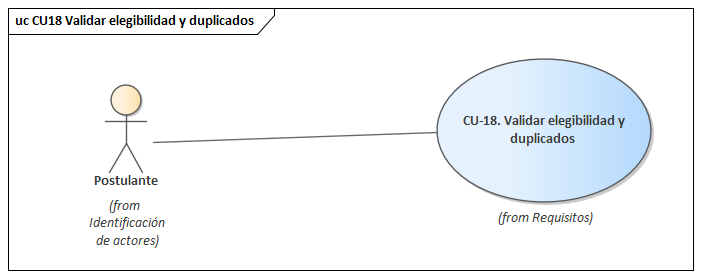
\includegraphics[width=0.8\textwidth,height=0.4\textheight,keepaspectratio]{images/047_CU18_Validar_Elegibilidad_Duplicados.png}

\smallskip
\noindent\raggedright\textit{Nota.} Elaboración propia.
\end{figure}

\refstepcounter{table}\label{tab:detalle_cu18}
\addcontentsline{lot}{table}{\protect\numberline{\thetable}Detalle del CU-18: Validar elegibilidad y duplicados}
\noindent\textbf{Tabla~\thetable}\par\nopagebreak
\noindent\textit{Detalle del CU-18: Validar elegibilidad y duplicados}\par\nopagebreak
\begingroup\small\linespread{1}\selectfont
\begin{longtable}{>{\raggedright\arraybackslash}p{2.9cm} >{\raggedright\arraybackslash}p{12.6cm}}
\toprule
\textbf{Caso de Uso} & \textbf{CU-18. Validar elegibilidad y duplicados} \\
\midrule
\endfirsthead
\toprule
\textbf{Caso de Uso} & \textbf{CU-18. Validar elegibilidad y duplicados} \\
\midrule
\endhead
\endfoot
\bottomrule
\multicolumn{2}{l}{\textit{Nota.} Elaboración propia.} \\
\endlastfoot
\textbf{Propósito} & Verificar, al momento de recibir una postulación, que el postulante cumple las condiciones de elegibilidad y que no existe otra postulación vigente suya en la misma gestión. \\
\midrule
\textbf{Descripción} & Este caso de uso describe la validación automática que ejecuta el sistema cuando el Postulante envía su postulación: comprueba las condiciones de elegibilidad definidas por la DUBSS y la unicidad de la postulación por postulante y gestión. Evita registros duplicados o inválidos que distorsionen la priorización y la adjudicación. Es incluido por el CU-02. Respalda el RF-13. \\
\midrule
\textbf{Actores} & Postulante. \\
\midrule
\textbf{Actor Iniciador} & Postulante (a través del CU-02, al enviar su postulación; el sistema ejecuta la validación). \\
\midrule
\textbf{Precondición} & \vspace{-\baselineskip}\begin{cuvin}
    \item El Postulante envió su postulación con los campos y documentos obligatorios completos (CU-02).
    \item Existe una convocatoria abierta a la que se asocia la postulación.
    \item Las condiciones de elegibilidad están configuradas en el sistema (por definir con la DUBSS).
\end{cuvin} \\
\midrule
\textbf{Proceso} & \textbf{Flujo principal.}
\begin{cupasos}
    \item El sistema recibe la solicitud de validación con la identidad del Postulante y la convocatoria de destino.
    \item El sistema consulta las postulaciones existentes del Postulante en la misma gestión académica.
    \item El sistema verifica que no exista otra postulación vigente del Postulante en la convocatoria.
    \item El sistema verifica las condiciones de elegibilidad (por ejemplo, la condición de estudiante de la UAGRM según su CI y perfil; reglas por definir con la DUBSS).
    \item El sistema devuelve al CU-02 el resultado «válida».
    \item El CU-02 continúa con el registro de la postulación.
\end{cupasos} \\
 & \textbf{Flujos alternativos.}
\begin{cuvin}
    \item A1 (paso 3): si ya existe otra postulación vigente del Postulante en la gestión, el sistema devuelve el resultado «duplicada» y el CU-02 rechaza el envío e informa el motivo.
    \item A2 (paso 4): si el Postulante no cumple alguna condición de elegibilidad, el sistema devuelve el resultado «no elegible» con el motivo específico, y el CU-02 rechaza el envío.
    \item A3 (paso 3): si se trata del reenvío de una postulación devuelta (CU-19), el sistema no la considera duplicada y la vincula con la postulación original, conservando el historial.
    \item A4 (paso 3): si se recibe una solicitud duplicada, el sistema devuelve el mismo resultado sin generar registros adicionales (idempotencia).
    \item A5 (paso 2): si el servicio de validación no está disponible, el sistema no acepta la postulación e informa al Postulante que reintente.
\end{cuvin} \\
\midrule
\textbf{Postcondición} & \vspace{-\baselineskip}\begin{cuvin}
    \item El sistema determina si la postulación es válida y, en caso afirmativo, el CU-02 puede registrarla.
    \item Si la postulación es rechazada, no se crea ningún registro y el Postulante recibe el motivo del rechazo.
\end{cuvin} \\
\midrule
\textbf{Excepciones} & \vspace{-\baselineskip}\begin{cuvin}
    \item Postulación duplicada en la misma gestión.
    \item Postulante no elegible según las condiciones establecidas.
    \item Servicio de validación no disponible.
    \item Error de conexión con el servidor o la base de datos.
\end{cuvin} \\
\end{longtable}
\endgroup
\addtocounter{table}{-1}

\subsubsection{5.4.19. CU-19 Devolver postulación para corrección}\label{sec:cap5_cu19}

\begin{figure}[H]
\caption{Diagrama de contexto del CU-19}
\label{fig:ctx_cu19}
\centering
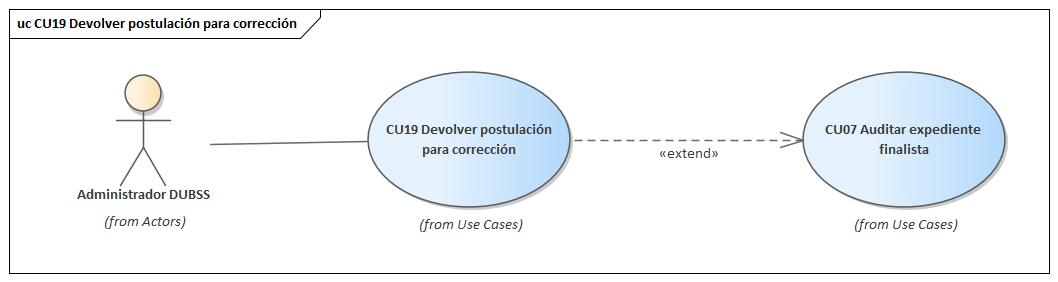
\includegraphics[width=0.8\textwidth,height=0.4\textheight,keepaspectratio]{images/072_CU19_Devolver_Postulacion_Correccion.jpg}

\smallskip
\noindent\raggedright\textit{Nota.} Elaboración propia.
\end{figure}

\refstepcounter{table}\label{tab:detalle_cu19}
\addcontentsline{lot}{table}{\protect\numberline{\thetable}Detalle del CU-19: Devolver postulación para corrección}
\noindent\textbf{Tabla~\thetable}\par\nopagebreak
\noindent\textit{Detalle del CU-19: Devolver postulación para corrección}\par\nopagebreak
\begingroup\small\linespread{1}\selectfont
\begin{longtable}{>{\raggedright\arraybackslash}p{2.9cm} >{\raggedright\arraybackslash}p{12.6cm}}
\toprule
\textbf{Caso de Uso} & \textbf{CU-19. Devolver postulación para corrección} \\
\midrule
\endfirsthead
\toprule
\textbf{Caso de Uso} & \textbf{CU-19. Devolver postulación para corrección} \\
\midrule
\endhead
\endfoot
\bottomrule
\multicolumn{2}{l}{\textit{Nota.} Elaboración propia.} \\
\endlastfoot
\textbf{Propósito} & Permitir al Administrador DUBSS devolver una postulación con observaciones para que el Postulante corrija o complete su documentación y la reenvíe, evitando descartarla por defectos subsanables. \\
\midrule
\textbf{Descripción} & Este caso de uso describe cómo el Administrador DUBSS, durante la auditoría de un expediente finalista, devuelve la postulación al Postulante registrando las observaciones que debe subsanar. La postulación cambia al estado «devuelta», el cambio queda en el historial de la postulación y el Postulante es notificado. El Postulante puede corregir y reenviar la postulación dentro del plazo establecido (por definir con la DUBSS) mediante el CU-02. Extiende el CU-07. Respalda el RF-14. \\
\midrule
\textbf{Actores} & Administrador DUBSS. \\
\midrule
\textbf{Actor Iniciador} & Administrador DUBSS. \\
\midrule
\textbf{Precondición} & \vspace{-\baselineskip}\begin{cuvin}
    \item El Administrador DUBSS está autenticado en el sistema (CU-01) con el rol Administrador DUBSS.
    \item El Administrador DUBSS se encuentra auditando el expediente de un finalista (CU-07).
    \item La postulación se encuentra en estado «calificada».
\end{cuvin} \\
\midrule
\textbf{Proceso} & \textbf{Flujo principal.}
\begin{cupasos}
    \item El Administrador DUBSS selecciona la opción «Devolver para corrección» en el expediente.
    \item El sistema solicita las observaciones de la devolución.
    \item El Administrador DUBSS registra las observaciones y confirma la devolución.
    \item El sistema valida que las observaciones no estén vacías.
    \item El sistema actualiza el estado de la postulación a «devuelta».
    \item El sistema registra el cambio en el historial de la postulación (estado anterior, estado nuevo, usuario y motivo) y en la bitácora.
    \item El sistema crea la notificación para el Postulante y le envía una notificación push con las observaciones.
    \item El sistema confirma la devolución al Administrador DUBSS.
\end{cupasos} \\
 & \textbf{Flujos alternativos.}
\begin{cuvin}
    \item A1 (paso 4): si no se registran observaciones, el sistema no permite devolver la postulación.
    \item A2 (paso 3): si el Administrador DUBSS cancela la operación, la postulación conserva su estado.
    \item A3 (paso 7): si falla el envío de la notificación push, la notificación queda registrada y el Postulante puede verla al consultar su postulación (CU-04).
    \item A4 (posterior al paso 8): cuando el Postulante corrige y reenvía la postulación (CU-02), esta vuelve al estado «pendiente», se incrementa su número de envíos y se conserva el historial de devoluciones y reenvíos.
\end{cuvin} \\
\midrule
\textbf{Postcondición} & \vspace{-\baselineskip}\begin{cuvin}
    \item La postulación queda en estado «devuelta» con las observaciones registradas en su historial.
    \item El Postulante es notificado y puede consultar las observaciones (CU-04).
\end{cuvin} \\
\midrule
\textbf{Excepciones} & \vspace{-\baselineskip}\begin{cuvin}
    \item Autenticación inválida o sesión expirada.
    \item Falta de permisos suficientes (el usuario no tiene el rol Administrador DUBSS).
    \item La postulación no se encuentra en un estado que permita su devolución.
    \item Error al enviar la notificación push mediante Firebase Cloud Messaging.
    \item Error de conexión con el servidor o la base de datos.
\end{cuvin} \\
\end{longtable}
\endgroup
\addtocounter{table}{-1}

\subsubsection{5.4.20. CU-20 Archivar o rechazar postulación}\label{sec:cap5_cu20}

\begin{figure}[H]
\caption{Diagrama de contexto del CU-20}
\label{fig:ctx_cu20}
\centering
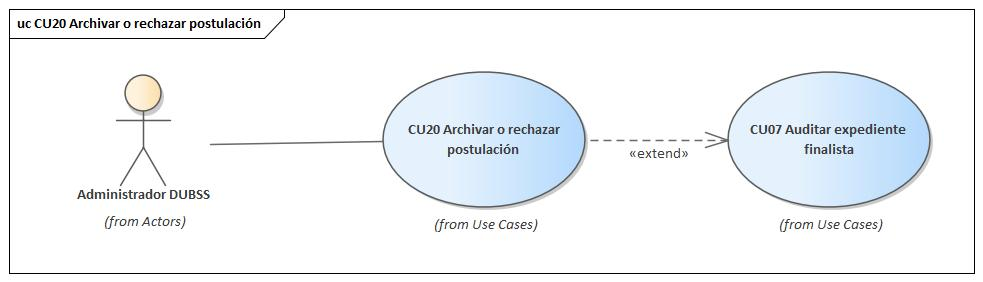
\includegraphics[width=0.8\textwidth,height=0.4\textheight,keepaspectratio]{images/073_CU20_Archivar_Rechazar_Postulacion.jpg}

\smallskip
\noindent\raggedright\textit{Nota.} Elaboración propia.
\end{figure}

\refstepcounter{table}\label{tab:detalle_cu20}
\addcontentsline{lot}{table}{\protect\numberline{\thetable}Detalle del CU-20: Archivar o rechazar postulación}
\noindent\textbf{Tabla~\thetable}\par\nopagebreak
\noindent\textit{Detalle del CU-20: Archivar o rechazar postulación}\par\nopagebreak
\begingroup\small\linespread{1}\selectfont
\begin{longtable}{>{\raggedright\arraybackslash}p{2.9cm} >{\raggedright\arraybackslash}p{12.6cm}}
\toprule
\textbf{Caso de Uso} & \textbf{CU-20. Archivar o rechazar postulación} \\
\midrule
\endfirsthead
\toprule
\textbf{Caso de Uso} & \textbf{CU-20. Archivar o rechazar postulación} \\
\midrule
\endhead
\endfoot
\bottomrule
\multicolumn{2}{l}{\textit{Nota.} Elaboración propia.} \\
\endlastfoot
\textbf{Propósito} & Permitir al Administrador DUBSS cerrar formalmente una postulación que no procede, archivándola o rechazándola, y dejar constancia del motivo de la decisión. \\
\midrule
\textbf{Descripción} & Este caso de uso describe cómo el Administrador DUBSS, durante la auditoría de un expediente finalista, archiva o rechaza una postulación registrando el motivo. Al archivarla, la postulación pasa al estado «archivada»; al rechazarla, pasa al estado «no adjudicada». En ambos casos deja de aparecer en la lista priorizada activa, el cambio queda en el historial de la postulación y esta se conserva para consulta histórica y reportes. Extiende el CU-07. Respalda el RF-15. \\
\midrule
\textbf{Actores} & Administrador DUBSS. \\
\midrule
\textbf{Actor Iniciador} & Administrador DUBSS. \\
\midrule
\textbf{Precondición} & \vspace{-\baselineskip}\begin{cuvin}
    \item El Administrador DUBSS está autenticado en el sistema (CU-01) con el rol Administrador DUBSS.
    \item El Administrador DUBSS se encuentra auditando el expediente de un finalista (CU-07).
    \item La postulación se encuentra en estado «calificada».
\end{cuvin} \\
\midrule
\textbf{Proceso} & \textbf{Flujo principal A: archivar la postulación.}
\begin{cupasos}
    \item El Administrador DUBSS selecciona la opción «Archivar» en el expediente.
    \item El sistema solicita el motivo del archivo.
    \item El Administrador DUBSS registra el motivo y confirma.
    \item El sistema valida que el motivo no esté vacío.
    \item El sistema actualiza el estado de la postulación a «archivada» y la retira de la lista priorizada activa.
    \item El sistema registra el cambio en el historial de la postulación (estado anterior, estado nuevo, usuario y motivo) y en la bitácora, y confirma la operación.
\end{cupasos} \\
 & \textbf{Flujo principal B: rechazar la postulación.}
\begin{cupasos}
    \item El Administrador DUBSS selecciona la opción «Rechazar» en el expediente.
    \item El sistema solicita el motivo del rechazo.
    \item El Administrador DUBSS registra el motivo y confirma.
    \item El sistema valida que el motivo no esté vacío.
    \item El sistema actualiza el estado de la postulación a «no adjudicada» y la retira de la lista priorizada activa.
    \item El sistema registra el cambio en el historial de la postulación (estado anterior, estado nuevo, usuario y motivo) y en la bitácora, y confirma la operación.
\end{cupasos} \\
 & \textbf{Flujos alternativos.}
\begin{cuvin}
    \item A1 (flujos A y B, paso 4): si no se registra el motivo, el sistema no permite completar la operación.
    \item A2 (flujos A y B, paso 3): si el Administrador DUBSS cancela la operación, la postulación conserva su estado.
    \item A3 (flujos A y B, paso 1): si la postulación ya se encuentra en un estado final («archivada», «adjudicada» o «no adjudicada») o los resultados de la convocatoria fueron publicados (CU-22), el sistema no permite la operación.
\end{cuvin} \\
\midrule
\textbf{Postcondición} & \vspace{-\baselineskip}\begin{cuvin}
    \item La postulación queda en estado «archivada» o «no adjudicada», con el motivo registrado en su historial, y se conserva para consulta histórica y reportes.
    \item El Postulante puede consultar el estado y el motivo registrado (CU-04).
\end{cuvin} \\
\midrule
\textbf{Excepciones} & \vspace{-\baselineskip}\begin{cuvin}
    \item Autenticación inválida o sesión expirada.
    \item Falta de permisos suficientes (el usuario no tiene el rol Administrador DUBSS).
    \item La postulación no se encuentra en un estado que permita archivarla o rechazarla.
    \item Error de conexión con el servidor o la base de datos.
\end{cuvin} \\
\end{longtable}
\endgroup
\addtocounter{table}{-1}

\subsubsection{5.4.21. CU-21 Notificar finalistas, registrar entrega de documentación física y publicar comunicados/avisos}\label{sec:cap5_cu21}

\begin{figure}[H]
\caption{Diagrama de contexto del CU-21}
\label{fig:ctx_cu21}
\centering
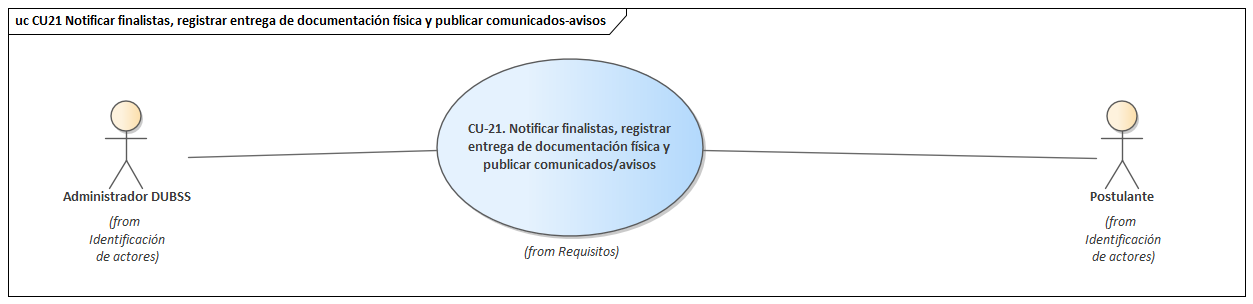
\includegraphics[width=0.8\textwidth,height=0.4\textheight,keepaspectratio]{images/048_CU21_Notificar_Finalistas_Publicar_Avisos.png}

\smallskip
\noindent\raggedright\textit{Nota.} Elaboración propia.
\end{figure}

\refstepcounter{table}\label{tab:detalle_cu21}
\addcontentsline{lot}{table}{\protect\numberline{\thetable}Detalle del CU-21: Notificar finalistas, registrar entrega de documentación física y publicar comunicados/avisos}
\noindent\textbf{Tabla~\thetable}\par\nopagebreak
\noindent\textit{Detalle del CU-21: Notificar finalistas, registrar entrega de documentación física y publicar comunicados/avisos}\par\nopagebreak
\begingroup\small\linespread{1}\selectfont
\begin{longtable}{>{\raggedright\arraybackslash}p{2.9cm} >{\raggedright\arraybackslash}p{12.6cm}}
\toprule
\textbf{Caso de Uso} & \textbf{CU-21. Notificar finalistas, registrar entrega de documentación física y publicar comunicados/avisos} \\
\midrule
\endfirsthead
\toprule
\textbf{Caso de Uso} & \textbf{CU-21. Notificar finalistas, registrar entrega de documentación física y publicar comunicados/avisos} \\
\midrule
\endhead
\endfoot
\bottomrule
\multicolumn{2}{l}{\textit{Nota.} Elaboración propia.} \\
\endlastfoot
\textbf{Propósito} & Permitir al Administrador DUBSS notificar a los finalistas para que presenten su documentación física, registrar su recepción y publicar comunicados y avisos dirigidos a los postulantes. \\
\midrule
\textbf{Descripción} & Este caso de uso agrupa tres funciones que coordinan la auditoría física: notificar a los finalistas el plazo y los documentos que deben presentar, registrar la fecha en que se recibe la documentación física de cada uno y publicar comunicados o avisos generales. Las notificaciones se envían mediante notificación push (Firebase Cloud Messaging) y quedan consultables en la aplicación. Es incluido por el CU-07 (Auditar expediente finalista). Respalda el RF-16. \\
\midrule
\textbf{Actores} & Administrador DUBSS; Postulante (receptor de las notificaciones). \\
\midrule
\textbf{Actor Iniciador} & Administrador DUBSS. \\
\midrule
\textbf{Precondición} & \vspace{-\baselineskip}\begin{cuvin}
    \item El Administrador DUBSS está autenticado en el sistema (CU-01) y cuenta con privilegios de administración.
    \item Para notificar finalistas y registrar entregas: existe una lista priorizada con finalistas definidos (CU-06), en el marco de la auditoría (CU-07).
    \item Para publicar comunicados: existe al menos un grupo de destinatarios (todos los postulantes o los finalistas).
\end{cuvin} \\
\midrule
\textbf{Proceso} & \textbf{Flujo principal A: notificar a los finalistas.}
\begin{cupasos}
    \item El Administrador accede a la gestión de finalistas desde la auditoría de expedientes (CU-07).
    \item El sistema muestra los finalistas de la lista priorizada (cantidad por definir con la DUBSS).
    \item El Administrador selecciona los finalistas a notificar (todos o un subconjunto) y define el plazo, el lugar y horario de entrega (por definir con la DUBSS) y los documentos físicos que deben presentar.
    \item El Administrador confirma el envío.
    \item El sistema envía una notificación push a cada finalista con el plazo y los documentos requeridos, y guarda el aviso en su bandeja de la aplicación.
    \item El sistema registra el envío (destinatarios, fecha y hora) en la bitácora (CU-25).
\end{cupasos} \\
 & \textbf{Flujo principal B: registrar la entrega de documentación física.}
\begin{cupasos}
    \item El Administrador busca al finalista por CI o nombre.
    \item El sistema muestra el expediente del finalista y el estado de su entrega (pendiente o recibida).
    \item El Administrador marca la documentación como recibida, indicando la fecha de recepción (por defecto, la fecha actual) y, opcionalmente, observaciones.
    \item El sistema guarda el registro y habilita la continuación de la auditoría del expediente (CU-07).
\end{cupasos} \\
 & \textbf{Flujo principal C: publicar comunicados y avisos.}
\begin{cupasos}
    \item El Administrador selecciona «Nuevo comunicado».
    \item El Administrador ingresa el título y el contenido, y elige los destinatarios (todos los postulantes o un grupo, por ejemplo los finalistas).
    \item El sistema muestra una vista previa y solicita confirmación.
    \item El Administrador confirma la publicación.
    \item El sistema publica el comunicado, envía una notificación push a los destinatarios, lo deja consultable en la aplicación y registra la acción en la bitácora.
\end{cupasos} \\
 & \textbf{Flujos alternativos.}
\begin{cuvin}
    \item A1 (flujo A, paso 5): si un finalista no tiene un dispositivo registrado para notificaciones push, el aviso queda disponible en su bandeja y se muestra al ingresar al sistema.
    \item A2 (flujo A, paso 5): si el envío push falla para algún destinatario, el sistema lo marca como fallido y permite reintentar el envío solo a esos destinatarios.
    \item A3 (flujo B, paso 3): si el finalista entrega la documentación de forma incompleta, el Administrador registra la observación y puede devolver la postulación (CU-19).
    \item A4 (flujo B, paso 3): si vence el plazo sin que el finalista entregue la documentación, el Administrador puede archivar o rechazar la postulación (CU-20).
    \item A5 (flujo B, paso 3): si el Administrador corrige una fecha de recepción ya registrada, el sistema conserva el valor anterior en la bitácora.
    \item A6 (flujo C, paso 2): si el título, el contenido o los destinatarios están vacíos, el sistema no permite la publicación e indica los campos faltantes.
\end{cuvin} \\
\midrule
\textbf{Postcondición} & \vspace{-\baselineskip}\begin{cuvin}
    \item Los finalistas notificados reciben el aviso con el plazo y los documentos requeridos.
    \item La recepción de la documentación física queda registrada con su fecha.
    \item Los comunicados publicados quedan consultables por los destinatarios desde la aplicación.
    \item Las acciones quedan registradas en la bitácora; esta funcionalidad no modifica el estado de la postulación.
\end{cuvin} \\
\midrule
\textbf{Excepciones} & \vspace{-\baselineskip}\begin{cuvin}
    \item Autenticación inválida o sesión expirada.
    \item Falta de permisos suficientes (el usuario no tiene el rol Administrador DUBSS).
    \item Datos ingresados no válidos o incompletos.
    \item Servicio de Firebase Cloud Messaging no disponible.
    \item Error de conexión con el servidor o la base de datos.
\end{cuvin} \\
\end{longtable}
\endgroup
\addtocounter{table}{-1}

\subsubsection{5.4.22. CU-22 Publicar resultados de adjudicación}\label{sec:cap5_cu22}

\begin{figure}[H]
\caption{Diagrama de contexto del CU-22}
\label{fig:ctx_cu22}
\centering
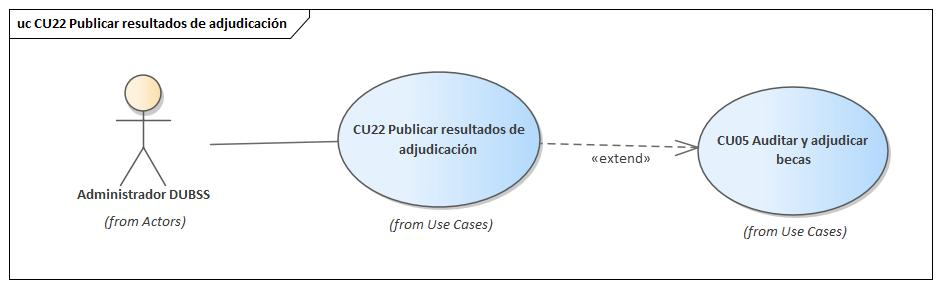
\includegraphics[width=0.8\textwidth,height=0.4\textheight,keepaspectratio]{images/074_CU22_Publicar_Resultados_Adjudicacion.jpg}

\smallskip
\noindent\raggedright\textit{Nota.} Elaboración propia.
\end{figure}

\refstepcounter{table}\label{tab:detalle_cu22}
\addcontentsline{lot}{table}{\protect\numberline{\thetable}Detalle del CU-22: Publicar resultados de adjudicación}
\noindent\textbf{Tabla~\thetable}\par\nopagebreak
\noindent\textit{Detalle del CU-22: Publicar resultados de adjudicación}\par\nopagebreak
\begingroup\small\linespread{1}\selectfont
\begin{longtable}{>{\raggedright\arraybackslash}p{2.9cm} >{\raggedright\arraybackslash}p{12.6cm}}
\toprule
\textbf{Caso de Uso} & \textbf{CU-22. Publicar resultados de adjudicación} \\
\midrule
\endfirsthead
\toprule
\textbf{Caso de Uso} & \textbf{CU-22. Publicar resultados de adjudicación} \\
\midrule
\endhead
\endfoot
\bottomrule
\multicolumn{2}{l}{\textit{Nota.} Elaboración propia.} \\
\endlastfoot
\textbf{Propósito} & Dar a conocer de forma oficial y transparente los resultados de la adjudicación de la Beca Comedor de una convocatoria y poner fin al proceso de selección. \\
\midrule
\textbf{Descripción} & Este caso de uso describe cómo el Administrador DUBSS, una vez decididas todas las adjudicaciones, publica la lista oficial de adjudicados de la convocatoria. Al publicar, el sistema registra la publicación y notifica a cada postulante su resultado mediante notificación push. La lista publicada es consultable por los postulantes y, desde ese momento, las adjudicaciones no se modifican sin dejar registro en la bitácora. Extiende el CU-05. Respalda el RF-17. \\
\midrule
\textbf{Actores} & Administrador DUBSS. \\
\midrule
\textbf{Actor Iniciador} & Administrador DUBSS. \\
\midrule
\textbf{Precondición} & \vspace{-\baselineskip}\begin{cuvin}
    \item El Administrador DUBSS está autenticado en el sistema (CU-01) con el rol Administrador DUBSS.
    \item Todas las adjudicaciones de los finalistas de la convocatoria están decididas (CU-05).
    \item Los resultados de la convocatoria no han sido publicados previamente.
\end{cuvin} \\
\midrule
\textbf{Proceso} & \textbf{Flujo principal.}
\begin{cupasos}
    \item El Administrador DUBSS selecciona la opción «Publicar resultados» de la convocatoria.
    \item El sistema obtiene y muestra las adjudicaciones de la convocatoria (adjudicados y no adjudicados) con el puntaje final de cada postulante.
    \item El Administrador DUBSS revisa los resultados y confirma la publicación.
    \item El sistema verifica que no existan adjudicaciones pendientes de decisión.
    \item El sistema registra la publicación con el usuario que la realiza y la fecha, y deja constancia en la bitácora.
    \item El sistema crea una notificación para cada postulante finalista con su resultado y le envía una notificación push.
    \item El sistema confirma la publicación; la lista de adjudicados queda consultable por los postulantes (CU-04).
\end{cupasos} \\
 & \textbf{Flujos alternativos.}
\begin{cuvin}
    \item A1 (paso 4): si existen adjudicaciones pendientes de decisión, el sistema no permite publicar e indica cuántas faltan.
    \item A2 (paso 1): si los resultados de la convocatoria ya fueron publicados, el sistema no permite una nueva publicación y muestra la existente.
    \item A3 (paso 6): si falla el envío de alguna notificación push, la notificación queda registrada y el postulante puede ver su resultado al consultar su postulación (CU-04).
    \item A4 (paso 3): si el Administrador DUBSS cancela la operación, no se publica ningún resultado.
\end{cuvin} \\
\midrule
\textbf{Postcondición} & \vspace{-\baselineskip}\begin{cuvin}
    \item Los resultados de la convocatoria quedan publicados y registrados con su responsable y fecha.
    \item Cada postulante finalista es notificado de su resultado y los adjudicados conforman el padrón de becados de la gestión (CU-23).
    \item Las adjudicaciones de la convocatoria no se modifican sin dejar registro en la bitácora (CU-25).
\end{cuvin} \\
\midrule
\textbf{Excepciones} & \vspace{-\baselineskip}\begin{cuvin}
    \item Autenticación inválida o sesión expirada.
    \item Falta de permisos suficientes (el usuario no tiene el rol Administrador DUBSS).
    \item Adjudicaciones pendientes de decisión.
    \item Error al enviar las notificaciones push mediante Firebase Cloud Messaging.
    \item Error de conexión con el servidor o la base de datos.
\end{cuvin} \\
\end{longtable}
\endgroup
\addtocounter{table}{-1}

\subsubsection{5.4.23. CU-23 Gestionar padrón de becados (baja, suspensión, reemplazo)}\label{sec:cap5_cu23}

\begin{figure}[H]
\caption{Diagrama de contexto del CU-23}
\label{fig:ctx_cu23}
\centering
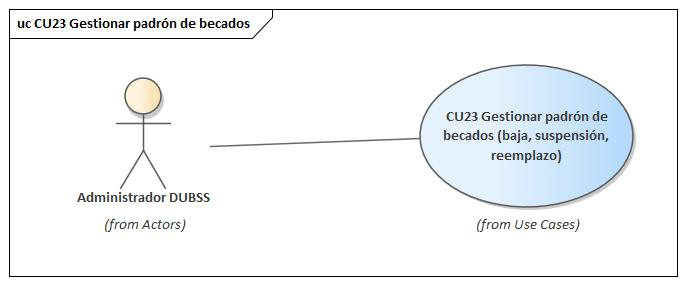
\includegraphics[width=0.8\textwidth,height=0.4\textheight,keepaspectratio]{images/075_CU23_Gestionar_Padron_Becados.jpg}

\smallskip
\noindent\raggedright\textit{Nota.} Elaboración propia.
\end{figure}

\refstepcounter{table}\label{tab:detalle_cu23}
\addcontentsline{lot}{table}{\protect\numberline{\thetable}Detalle del CU-23: Gestionar padrón de becados (baja, suspensión, reemplazo)}
\noindent\textbf{Tabla~\thetable}\par\nopagebreak
\noindent\textit{Detalle del CU-23: Gestionar padrón de becados (baja, suspensión, reemplazo)}\par\nopagebreak
\begingroup\small\linespread{1}\selectfont
\begin{longtable}{>{\raggedright\arraybackslash}p{2.9cm} >{\raggedright\arraybackslash}p{12.6cm}}
\toprule
\textbf{Caso de Uso} & \textbf{CU-23. Gestionar padrón de becados (baja, suspensión, reemplazo)} \\
\midrule
\endfirsthead
\toprule
\textbf{Caso de Uso} & \textbf{CU-23. Gestionar padrón de becados (baja, suspensión, reemplazo)} \\
\midrule
\endhead
\endfoot
\bottomrule
\multicolumn{2}{l}{\textit{Nota.} Elaboración propia.} \\
\endlastfoot
\textbf{Propósito} & Mantener actualizado el padrón de becados vigentes de la gestión, registrando bajas, suspensiones y reemplazos, del cual dependen las planillas de asistencia. \\
\midrule
\textbf{Descripción} & Este caso de uso describe cómo el Administrador DUBSS consulta el padrón de becados de una convocatoria y registra sobre él las bajas, suspensiones y reemplazos que ocurren durante la gestión. Cada cambio actualiza el estado de la beca y queda registrado como un movimiento con su motivo, responsable y fecha. En un reemplazo, el cupo liberado se asigna al siguiente postulante priorizado. Los cambios se reflejan en las planillas de asistencia generadas posteriormente (CU-09). Respalda el RF-18. \\
\midrule
\textbf{Actores} & Administrador DUBSS. \\
\midrule
\textbf{Actor Iniciador} & Administrador DUBSS. \\
\midrule
\textbf{Precondición} & \vspace{-\baselineskip}\begin{cuvin}
    \item El Administrador DUBSS está autenticado en el sistema (CU-01) con el rol Administrador DUBSS.
    \item Los resultados de adjudicación de la convocatoria fueron publicados (CU-22) y existen becas registradas.
\end{cuvin} \\
\midrule
\textbf{Proceso} & \textbf{Flujo principal A: consultar el padrón.}
\begin{cupasos}
    \item El Administrador DUBSS selecciona la opción «Padrón de becados» y la convocatoria.
    \item El sistema muestra las becas de la convocatoria con el nombre, CI y carrera del becado y el estado de la beca (vigente, suspendida o baja).
\end{cupasos} \\
 & \textbf{Flujo principal B: dar de baja o suspender una beca.}
\begin{cupasos}
    \item El Administrador DUBSS selecciona una beca vigente y la opción «Dar de baja» o «Suspender».
    \item El sistema solicita el motivo.
    \item El Administrador DUBSS registra el motivo y confirma.
    \item El sistema actualiza el estado de la beca a «baja» o «suspendida», según corresponda.
    \item El sistema registra el movimiento (tipo, motivo, usuario y fecha) y deja constancia en la bitácora.
\end{cupasos} \\
 & \textbf{Flujo principal C: reemplazar un cupo liberado.}
\begin{cupasos}
    \item El Administrador DUBSS selecciona una beca dada de baja y la opción «Reemplazar».
    \item El sistema muestra al siguiente postulante de la lista priorizada disponible para ocupar el cupo.
    \item El Administrador DUBSS confirma el reemplazo.
    \item El sistema crea una nueva beca vigente para el postulante reemplazante.
    \item El sistema registra el movimiento de reemplazo, vinculando la beca liberada con la beca reemplazante, y deja constancia en la bitácora.
\end{cupasos} \\
 & \textbf{Flujos alternativos.}
\begin{cuvin}
    \item A1 (flujo B, paso 3): si no se registra el motivo, el sistema no permite completar la operación.
    \item A2 (flujo B, paso 1): si la beca no está vigente, el sistema no permite darla de baja ni suspenderla.
    \item A3 (flujo C, paso 1): si la beca seleccionada no ha sido dada de baja, el sistema no permite el reemplazo.
    \item A4 (flujo C, paso 2): si no existe un postulante disponible para ocupar el cupo, el sistema lo informa y no realiza el reemplazo.
    \item A5 (flujos B y C): si el Administrador DUBSS cancela la operación, el padrón no se modifica.
\end{cuvin} \\
\midrule
\textbf{Postcondición} & \vspace{-\baselineskip}\begin{cuvin}
    \item El padrón refleja el estado actualizado de cada beca y cada cambio queda registrado como movimiento y en la bitácora.
    \item Las planillas de asistencia que se generen posteriormente (CU-09) consideran solo las becas vigentes.
\end{cuvin} \\
\midrule
\textbf{Excepciones} & \vspace{-\baselineskip}\begin{cuvin}
    \item Autenticación inválida o sesión expirada.
    \item Falta de permisos suficientes (el usuario no tiene el rol Administrador DUBSS).
    \item Operación no permitida para el estado actual de la beca.
    \item Error de conexión con el servidor o la base de datos.
\end{cuvin} \\
\end{longtable}
\endgroup
\addtocounter{table}{-1}

\subsubsection{5.4.24. CU-24 Consultar historial de asistencia y estado de beca}\label{sec:cap5_cu24}

\begin{figure}[H]
\caption{Diagrama de contexto del CU-24}
\label{fig:ctx_cu24}
\centering
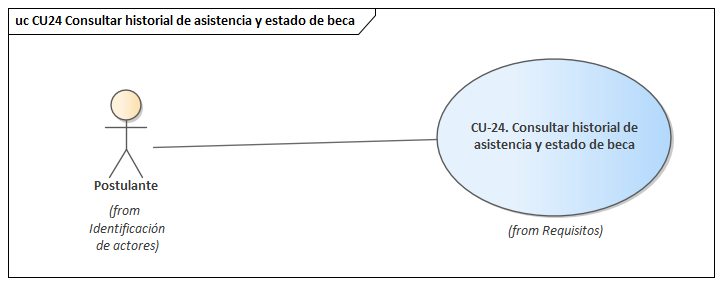
\includegraphics[width=0.8\textwidth,height=0.4\textheight,keepaspectratio]{images/049_CU24_Consultar_Historial_Asistencia_Beca.png}

\smallskip
\noindent\raggedright\textit{Nota.} Elaboración propia.
\end{figure}

\refstepcounter{table}\label{tab:detalle_cu24}
\addcontentsline{lot}{table}{\protect\numberline{\thetable}Detalle del CU-24: Consultar historial de asistencia y estado de beca}
\noindent\textbf{Tabla~\thetable}\par\nopagebreak
\noindent\textit{Detalle del CU-24: Consultar historial de asistencia y estado de beca}\par\nopagebreak
\begingroup\small\linespread{1}\selectfont
\begin{longtable}{>{\raggedright\arraybackslash}p{2.9cm} >{\raggedright\arraybackslash}p{12.6cm}}
\toprule
\textbf{Caso de Uso} & \textbf{CU-24. Consultar historial de asistencia y estado de beca} \\
\midrule
\endfirsthead
\toprule
\textbf{Caso de Uso} & \textbf{CU-24. Consultar historial de asistencia y estado de beca} \\
\midrule
\endhead
\endfoot
\bottomrule
\multicolumn{2}{l}{\textit{Nota.} Elaboración propia.} \\
\endlastfoot
\textbf{Propósito} & Permitir al Postulante adjudicado (becado) consultar su historial de asistencia al comedor y el estado vigente de su beca. \\
\midrule
\textbf{Descripción} & Este caso de uso describe cómo el becado consulta, desde el portal web o la aplicación móvil, las fechas de asistencia registradas en la gestión vigente y el estado de su beca (vigente, suspendida o dada de baja) con su motivo, de modo que pueda verificar el cumplimiento de los requisitos de asistencia y conservar su beneficio. Es una consulta de solo lectura que utiliza los datos registrados en el CU-10 y en el padrón de becados (CU-23). Respalda el RF-19. \\
\midrule
\textbf{Actores} & Postulante (becado, es decir, Postulante adjudicado). \\
\midrule
\textbf{Actor Iniciador} & Postulante (becado). \\
\midrule
\textbf{Precondición} & \vspace{-\baselineskip}\begin{cuvin}
    \item El Postulante está autenticado en el sistema (CU-01).
    \item La postulación del Postulante fue adjudicada y figura en el padrón de becados.
\end{cuvin} \\
\midrule
\textbf{Proceso} & \textbf{Flujo principal.}
\begin{cupasos}
    \item El becado accede a la opción «Mi beca».
    \item El sistema verifica que el usuario figure en el padrón de becados de la gestión.
    \item El sistema muestra el estado de la beca (vigente, suspendida o dada de baja), la gestión académica y la fecha de adjudicación.
    \item El sistema muestra el historial de asistencia de la gestión vigente: las fechas de asistencia registradas en el comedor y el total acumulado.
    \item El becado revisa la información y, opcionalmente, filtra el historial por rango de fechas.
\end{cupasos} \\
 & \textbf{Flujos alternativos.}
\begin{cuvin}
    \item A1 (paso 2): si el usuario no figura como becado, el sistema informa que no cuenta con una beca vigente y lo redirige a la consulta del estado de su postulación (CU-04).
    \item A2 (paso 4): si aún no existen asistencias registradas, el sistema muestra un mensaje informativo.
    \item A3 (paso 3): si la beca está suspendida o dada de baja, el sistema muestra el estado y el motivo registrado por el Administrador (CU-23); el historial de asistencia se conserva y sigue siendo consultable.
    \item A4 (paso 1): si el usuario intenta acceder a la información de otro becado, el sistema deniega el acceso.
\end{cuvin} \\
\midrule
\textbf{Postcondición} & \vspace{-\baselineskip}\begin{cuvin}
    \item El becado visualiza su historial de asistencia y el estado de su beca; la consulta no modifica ningún dato del sistema.
\end{cuvin} \\
\midrule
\textbf{Excepciones} & \vspace{-\baselineskip}\begin{cuvin}
    \item Autenticación inválida o sesión expirada.
    \item Falta de permisos suficientes (el usuario solo puede acceder a su propia información).
    \item Usuario sin beca adjudicada.
    \item Error de conexión con el servidor o la base de datos.
\end{cuvin} \\
\end{longtable}
\endgroup
\addtocounter{table}{-1}

\subsubsection{5.4.25. CU-25 Consultar bitácora de acciones}\label{sec:cap5_cu25}

\begin{figure}[H]
\caption{Diagrama de contexto del CU-25}
\label{fig:ctx_cu25}
\centering
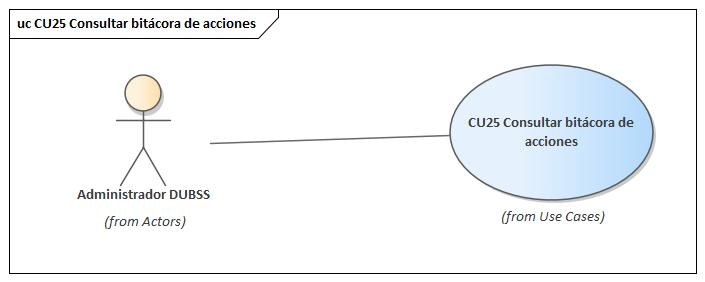
\includegraphics[width=0.8\textwidth,height=0.4\textheight,keepaspectratio]{images/076_CU25_Consultar_Bitacora_Acciones.jpg}

\smallskip
\noindent\raggedright\textit{Nota.} Elaboración propia.
\end{figure}

\refstepcounter{table}\label{tab:detalle_cu25}
\addcontentsline{lot}{table}{\protect\numberline{\thetable}Detalle del CU-25: Consultar bitácora de acciones}
\noindent\textbf{Tabla~\thetable}\par\nopagebreak
\noindent\textit{Detalle del CU-25: Consultar bitácora de acciones}\par\nopagebreak
\begingroup\small\linespread{1}\selectfont
\begin{longtable}{>{\raggedright\arraybackslash}p{2.9cm} >{\raggedright\arraybackslash}p{12.6cm}}
\toprule
\textbf{Caso de Uso} & \textbf{CU-25. Consultar bitácora de acciones} \\
\midrule
\endfirsthead
\toprule
\textbf{Caso de Uso} & \textbf{CU-25. Consultar bitácora de acciones} \\
\midrule
\endhead
\endfoot
\bottomrule
\multicolumn{2}{l}{\textit{Nota.} Elaboración propia.} \\
\endlastfoot
\textbf{Propósito} & Permitir al Administrador DUBSS consultar el registro de las acciones relevantes realizadas en el sistema, para garantizar la trazabilidad de las decisiones y facilitar las auditorías. \\
\midrule
\textbf{Descripción} & Este caso de uso describe cómo el Administrador DUBSS consulta la bitácora del sistema, en la que se registran automáticamente las acciones relevantes (auditoría, devolución, adjudicación, publicación, cambios en el padrón y cambios de roles) con el usuario, la acción, la entidad o expediente afectado, la fecha y la hora. La bitácora puede filtrarse por usuario, tipo de acción y rango de fechas. Es una consulta de solo lectura: los registros no pueden editarse ni eliminarse. Respalda el RF-20. \\
\midrule
\textbf{Actores} & Administrador DUBSS. \\
\midrule
\textbf{Actor Iniciador} & Administrador DUBSS. \\
\midrule
\textbf{Precondición} & \vspace{-\baselineskip}\begin{cuvin}
    \item El Administrador DUBSS está autenticado en el sistema (CU-01) con el rol Administrador DUBSS.
\end{cuvin} \\
\midrule
\textbf{Proceso} & \textbf{Flujo principal.}
\begin{cupasos}
    \item El Administrador DUBSS selecciona la opción «Bitácora de acciones».
    \item El sistema muestra los registros de la bitácora ordenados del más reciente al más antiguo y paginados, con la fecha y hora, el usuario, la acción, la entidad o expediente afectado y el detalle de cada registro.
    \item El Administrador DUBSS ingresa los filtros de búsqueda: usuario, tipo de acción y rango de fechas.
    \item El sistema muestra los registros que cumplen los filtros.
\end{cupasos} \\
 & \textbf{Flujos alternativos.}
\begin{cuvin}
    \item A1 (paso 4): si ningún registro cumple los filtros, el sistema muestra un mensaje informativo.
    \item A2 (paso 3): si la fecha final del rango es anterior a la inicial, el sistema lo indica y permite corregirla.
    \item A3 (paso 2): las acciones ejecutadas por el sistema o por el módulo de IA se muestran sin usuario asociado.
\end{cuvin} \\
\midrule
\textbf{Postcondición} & \vspace{-\baselineskip}\begin{cuvin}
    \item El Administrador DUBSS visualiza los registros de la bitácora; la consulta no modifica ningún dato del sistema.
\end{cuvin} \\
\midrule
\textbf{Excepciones} & \vspace{-\baselineskip}\begin{cuvin}
    \item Autenticación inválida o sesión expirada.
    \item Falta de permisos suficientes (el usuario no tiene el rol Administrador DUBSS).
    \item Error de conexión con el servidor o la base de datos.
\end{cuvin} \\
\end{longtable}
\endgroup
\addtocounter{table}{-1}

\subsubsection{5.4.26. CU-26 Parametrizar modelo de preselección y reprocesar puntajes}\label{sec:cap5_cu26}

\begin{figure}[H]
\caption{Diagrama de contexto del CU-26}
\label{fig:ctx_cu26}
\centering
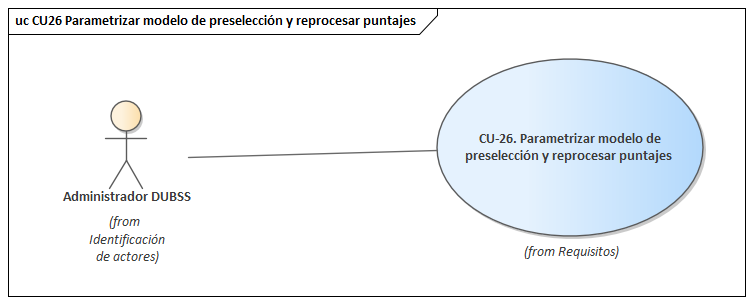
\includegraphics[width=0.8\textwidth,height=0.4\textheight,keepaspectratio]{images/050_CU26_Parametrizar_Modelo_Preseleccion.png}

\smallskip
\noindent\raggedright\textit{Nota.} Elaboración propia.
\end{figure}

\refstepcounter{table}\label{tab:detalle_cu26}
\addcontentsline{lot}{table}{\protect\numberline{\thetable}Detalle del CU-26: Parametrizar modelo de preselección y reprocesar puntajes}
\noindent\textbf{Tabla~\thetable}\par\nopagebreak
\noindent\textit{Detalle del CU-26: Parametrizar modelo de preselección y reprocesar puntajes}\par\nopagebreak
\begingroup\small\linespread{1}\selectfont
\begin{longtable}{>{\raggedright\arraybackslash}p{2.9cm} >{\raggedright\arraybackslash}p{12.6cm}}
\toprule
\textbf{Caso de Uso} & \textbf{CU-26. Parametrizar modelo de preselección y reprocesar puntajes} \\
\midrule
\endfirsthead
\toprule
\textbf{Caso de Uso} & \textbf{CU-26. Parametrizar modelo de preselección y reprocesar puntajes} \\
\midrule
\endhead
\endfoot
\bottomrule
\multicolumn{2}{l}{\textit{Nota.} Elaboración propia.} \\
\endlastfoot
\textbf{Propósito} & Permitir al Administrador DUBSS ajustar los criterios y ponderaciones del modelo de preselección y reprocesar los puntajes de las postulaciones de una convocatoria. \\
\midrule
\textbf{Descripción} & Este caso de uso describe cómo el Administrador DUBSS consulta y modifica los parámetros del modelo de IA (criterios y ponderaciones de las variables socioeconómicas y académicas), los guarda como una nueva versión y, si lo decide, reprocesa los puntajes de una convocatoria. Cada recálculo conserva el puntaje anterior para fines de trazabilidad. Extiende al CU-03. Respalda el RF-21. \\
\midrule
\textbf{Actores} & Administrador DUBSS. \\
\midrule
\textbf{Actor Iniciador} & Administrador DUBSS. \\
\midrule
\textbf{Precondición} & \vspace{-\baselineskip}\begin{cuvin}
    \item El Administrador DUBSS está autenticado en el sistema (CU-01) y cuenta con privilegios de administración.
    \item El módulo de IA está disponible.
    \item Para reprocesar: la convocatoria seleccionada tiene postulaciones precalificadas (CU-03).
\end{cuvin} \\
\midrule
\textbf{Proceso} & \textbf{Flujo principal.}
\begin{cupasos}
    \item El Administrador accede a la opción «Parámetros del modelo».
    \item El sistema muestra los criterios y ponderaciones vigentes (variables: ingresos familiares, dependientes, procedencia, carrera, patrimonio, estado de vulnerabilidad y promedio académico), con su versión y fecha de vigencia.
    \item El Administrador modifica los criterios o ponderaciones necesarios (valores y rangos por definir con la DUBSS).
    \item El sistema valida los valores ingresados (rangos permitidos y consistencia entre ponderaciones).
    \item El Administrador guarda los cambios y el sistema crea una nueva versión de los parámetros, conservando las versiones anteriores.
    \item El Administrador selecciona la convocatoria y solicita «Reprocesar puntajes».
    \item El sistema muestra el resumen del reprocesamiento (convocatoria y cantidad de postulaciones afectadas) y solicita confirmación.
    \item El Administrador confirma.
    \item El sistema ejecuta el reprocesamiento en lote, invocando el cálculo del CU-03 para cada postulación, y muestra el avance.
    \item El sistema registra la fecha de cada recálculo y conserva el puntaje anterior de cada postulación.
    \item El sistema muestra la lista priorizada actualizada (CU-06) y registra la acción en la bitácora (CU-25).
\end{cupasos} \\
 & \textbf{Flujos alternativos.}
\begin{cuvin}
    \item A1 (paso 4): si los valores están fuera de rango o son inconsistentes, el sistema indica los errores y no guarda los parámetros.
    \item A2 (paso 5): si el Administrador guarda los parámetros sin reprocesar, la nueva versión se aplica únicamente a las postulaciones que se precalifiquen a partir de ese momento.
    \item A3 (paso 6): si ya se publicaron resultados de adjudicación en la convocatoria (CU-22), el sistema advierte o bloquea el reprocesamiento (regla por definir con la DUBSS).
    \item A4 (paso 6): si hay un reprocesamiento en curso para la misma convocatoria, el sistema impide lanzar otro de forma simultánea.
    \item A5 (paso 9): si el cálculo falla para algunas postulaciones, el sistema continúa con las demás, lista las fallidas y permite reintentarlas.
    \item A6 (paso 7): el Administrador puede cancelar el reprocesamiento antes de confirmarlo, sin que se modifique ningún puntaje.
\end{cuvin} \\
\midrule
\textbf{Postcondición} & \vspace{-\baselineskip}\begin{cuvin}
    \item Los nuevos parámetros quedan guardados como una versión vigente, y las versiones anteriores se conservan.
    \item Los puntajes reprocesados quedan registrados con su fecha de recálculo y el puntaje anterior se conserva; la lista priorizada refleja el nuevo orden.
    \item La acción queda registrada en la bitácora.
\end{cuvin} \\
\midrule
\textbf{Excepciones} & \vspace{-\baselineskip}\begin{cuvin}
    \item Autenticación inválida o sesión expirada.
    \item Falta de permisos suficientes (el usuario no tiene el rol Administrador DUBSS).
    \item Parámetros ingresados no válidos.
    \item Módulo de IA no disponible durante el reprocesamiento.
    \item Error de conexión con el servidor o la base de datos.
\end{cuvin} \\
\end{longtable}
\endgroup
\addtocounter{table}{-1}
